%Inicio do Pre\^{a}mbulo

\documentclass[12pt,openright,oneside,a4paper,brazil]{abntex2}
%normaltoc - coloca o 
%normalfigtabnum
% Pacotes básicos 
% ---
\usepackage{lmodern}			% Usa a fonte Latin Modern			
\usepackage[T1]{fontenc}		% Selecao de codigos de fonte.
\usepackage[utf8]{inputenc}		% Codificacao do documento (conversão automática dos acentos)
\usepackage{lastpage}			% Usado pela Ficha catalográfica
\usepackage{indentfirst}		% Indenta o primeiro parágrafo de cada seção.
\usepackage{color}				% Controle das cores
\usepackage{graphicx}			% Inclusão de gráficos
\usepackage{textcomp}
%\usepackage[brazilian,hyperpageref]{backref}	 % Paginas com as citações na bibl
\usepackage[alf]{abntex2cite}	% Citações padrão ABNT
\usepackage{multirow}
\usepackage{microtype} 			% para melhorias de justificaçãoo
%\usepackage[latin1]{inputenc}
% ---
%Anteriores
%\usepackage[brazil]{babel}
%\usepackage[ansinew]{inputenc}
%\usepackage[T1]{fontenc}
%\usepackage{graphicx} %pacote para figuras JPGE para inserir figuras no texto
%\usepackage[alf,abnt-full-initials=yes,abnt-etal-text=it]{abntcite}

% Pacotes adicionais, usados apenas no âmbito do Modelo Canônico do abnteX2
% ---
%\usepackage{lipsum}				% para geração de dummy text (texto fictício)
% ---

% ---
% Configurações do pacote backref
% Usado sem a opção hyperpageref de backref
%\renewcommand{\backrefpagesname}{Citado na(s) página(s):~}
% Texto padrão antes do número das páginas
%\renewcommand{\backref}{}
% Define os textos da citação
%\renewcommand*{\backrefalt}[4]{
%	\ifcase #1 %
%		Nenhuma citação no texto.%
%	\or
%		Citado na página #2.%
%	\else
%		Citado #1 vezes nas páginas #2.%
% 	\fi}%
% ---
% =========  FIM Configurações para informar paginas onde ocorreram citações de autor na referencia ================

% ---

% informações do PDF
\makeatletter
\hypersetup{
     	%pagebackref=true,
		pdftitle={\@title}, 
		pdfauthor={\@author},
    	pdfsubject={\imprimirpreambulo},
	    pdfcreator={LaTeX with abnTeX2},
		pdfkeywords={abnt}{latex}{abntex}{abntex2}{trabalho acadêmico}, 
		colorlinks=true,       		% false: boxed links; true: colored links
    	linkcolor=black,        %linkcolor=blue,       	% color of internal links
    	citecolor=black,        %citecolor=blue,    		% color of links to bibliography
    	filecolor=magenta,                          		% color of file links
		urlcolor=black,           %urlcolor=blue,
		bookmarksdepth=4
}
\makeatother
% --- 

% O tamanho do parágrafo é dado por:
\setlength{\parindent}{1.3cm}

% Controle do espaçamento entre um parágrafo e outro:
\setlength{\parskip}{0.2cm}  % tente também \onelineskip

% ---
% compila o indice
% ---
\makeindex
% ---

\def \b{$\bullet$}
%\renewcommand{\ABNTchapterfont}{\bfseries\selectfont}% Alterar fonte dos capitulos para Times New Roman
%\renewcommand{\ABNTsectionfont}{\bfseries\selectfont}% Alterar fonte das secoes/subsecoes para Times New Roman
%\setlength{\parindent}{1.5cm} %recuo de paragrafo

\begin{document}
%\renewcommand{\apudname}{\textit{apud}} % Colocar apud em italico

% Retira espaço extra obsoleto entre as frases.
\frenchspacing 

%======================= CAPA E FOLHA DE ROSTO =============================
%\begin{titlepage}%ambiente que permite a criação de uma capa própria
\begin{center}   %modo centralizado

\begin{figure}[h] %h insere a figura onde ela está no texto
\centering        %centraliza a figura

\includegraphics[width=7.0cm, height=3.0cm]{imagens/UNIGRAN.jpg} %define o
% tamanho da figura
\end{figure}      %encerra modo figura

\textbf{CENTRO UNIVERSITÁRIO DA GRANDE DOURADOS}

\begin{figure}[h]
\centering

\includegraphics[width=15.0cm, height=0.40cm]{imagens/AMARELO.jpg}
\end{figure}

\textbf{MARCELO BENTO PEREIRA} 
\\

\vspace{5cm}%define os espaços entre as frases de 7 centímetros

\textbf{TELEFONIA VoIP: UMA PROPOSTA DE MELHORIA DO TELEATENDIMENTO EMERGENCIAL DA POLÍCIA MILITAR DE DOURADOS UTILIZANDO PABX IP} %\textbf Texto em negrito

\vspace{10cm}

\begin{figure}[h]
\centering

\includegraphics[width=15.0cm, height=0.40cm]{imagens/AZUL.jpg}

\end{figure}

\textbf{Dourados}
\vspace{-0,5cm} %diminue os espaço entre as frases em 0,5 centímetros a menos que o normal

\textbf{2015}

\end{center}%encerra modo centralizado
%\end{titlepage}%encerra modo de capa

%\begin{titlepage}%ambiente que permite a criação de uma capa própria
\begin{center}   %modo centralizado

\begin{figure}[h] %h insere a figura onde ela está no texto
\centering        %centraliza a figura

\includegraphics[width=7.0cm, height=3.0cm]{imagens/UNIGRAN.jpg} %define o
% tamanho da figura
\end{figure}      %encerra modo figura

\textbf{CENTRO UNIVERSITÁRIO DA GRANDE DOURADOS}

\begin{figure}[h]
\centering

\includegraphics[width=15.0cm, height=0.40cm]{imagens/AMARELO.jpg}
\end{figure}

% \hspace{\fill} justifica a esquerda o texto anterior e a direita o posterior

\textbf{MARCELO BENTO PEREIRA}  \\ 
% \textbf{NOME DO OUTRO ALUNO}

\vspace{4cm}

\textbf{VOZ SOBRE IP: UMA PROPOSTA DE MELHORIA DO TELEATENDIMENTO EMERGENCIAL DA POLÍCIA MILITAR DE DOURADOS UTILIZANDO PABX IP}  % Texto em Negrito

\vspace{2cm}

\begin{flushright}  % ajustar o texto a direita
\parbox[c]{.5\linewidth}{
            Trabalho de conclusão de curso apresentado ao Curso de Ciência da Computação da Faculdade de Ciências Exatas e da Terra do Centro Universitário da Grande Dourados, como pré-requisito para obtenção do título de Bacharel em Ciência da Computação.
            \vspace{1cm}

            Orientador: Felipe Pereira Perez.
         }
\end{flushright}

\vspace{1cm}

\begin{figure}[h]
\centering

\includegraphics[width=15.0cm, height=0.40cm]{imagens/AZUL.jpg}\
\end{figure}

\textbf{Dourados}

\vspace{-0,5cm} % diminue os espaço entre as frases em 0,5 centímetros a menos que o normal

\textbf{2015}

\end{center}%encerra modo centralizado
%\end{titlepage}%encerra modo de capa

%======================= RESUMO =============================
%\pagenumbering{roman}
\setlength{\absparsep}{18pt} % ajusta o espaçamento dos parágrafos do resumo
\begin{resumo}

Este trabalho tem como objetivo proporcionar uma melhoria no teleatendimento emergencial da Polícia Militar de Dourados, sendo que este trabalho consiste na investigação e apresentação de possíveis falhas técnicas ou mesmo humanas, mas para isso sera apresentados conceitos referentes à ambientes de telefonia, a fim de desenvolver um ambiente propício para protótipo funcional de um servidor PABX com emprego da tecnologia de transmissão de voz sobre IP, mais precisamente a ferramenta Asterisk e gama de serviços que esta possui, porém o foco principal é nas melhorias técnicas que esta ferramenta tem a proporcionar, e coerentemente trará benefícios nos recursos humanos deste teleatendimento.

 \textbf{Palavras-chaves}: \textit{VoIP. PSTN. Teleatendimento. Agregação de Serviços a Telefonia.}.
\end{resumo}

%\clearpage

%======================= LISTA DE FIGURAS =============================
% ---
% inserir lista de ilustrações
% ---
\pdfbookmark[0]{\listfigurename}{lof}
\listoffigures*
\cleardoublepage
% ---

%========================LISTA DE TABELAS =============================
% inserir lista de tabelas
% ---

%\pdfbookmark[0]{\listtablename}{lot}

%\listoftables*

%\clearpage
%\cleardoublepage
% ---

% ---
% inserir lista de abreviaturas e siglas
% ---
\begin{siglas}
  \item[ANI]	 \textit{Automatic Idendification Number}
  \item[CAS]	 \textit{Channel Associated Singalling}
  \item[CCS]	 \textit{Commom Chanel Signalling}
  \item[DNIS]	 \textit{Dialed Number Identification Service}
  \item[DTMF]	 \textit{Dual-Tone Multri Frequency}
  \item[IP]		 \textit{Internet Protocol}
  \item[ISDN]	 \textit{Integrated Service Digital Network}
  \item[MFC]	 \textit{Multi-Frequency Compelido}
  \item[ODBC]	 \textit{Open Database Connectivity}
  \item[PABX]	 \textit{Private Automatic Branch eXchange}
  \item[PABX IP] \textit{Private Automatic Branch eXchange Internet Protocol}
  \item[PCM]	 \textit{Pulse Code Modelation}
  \item[PRI]	 \textit{Primary Rate Interface}
  \item[PSTN]	 \textit{Public Service Telephony Network}
  \item[RDSI]	 \textit{Rede Digital de Serviços Integrada}
  \item[RTPC]	 \textit{Rede de Tefefonia Pública Comutada}
  \item[SGDB]	 \textit{Sistema de Gerenciamento de Banco de Dados}
  \item[SS7]	 \textit{Signaling System 7}
  \item[TDM]	 \textit{Time-Division Multiplexing}
  \item[VoIP]	 \textit{Voice over Internet Protocol}
\end{siglas}
% ---

%======================= LISTA DE SIGLAS ==============================
%\chapter*{Lista de siglas}
%\begin{tabular}{lll}
%	ANI     & & {\em Automatic Idendification Number} \\
%	CAS     & & {\em Channel Associated Singalling} \\
%	CCS     & & {\em Commom Chanel Signalling} \\
%	DNIS     & & {\em Dialed Number Identification Service} \\
%	DTMF     & & {\em Dual-Tone Multri Frequency} \\
%	IP     & & {\em Internet Protocol} \\
%	ISDN     & & {\em Integrated Service Digital Network} \\
%	MFC     & & {\em Multi-Frequency Compelido} \\
%	ODBC     & & {\em Open Database Connectivity} \\
%	PABX     & & {\em Private Automatic Branch eXchange} \\
%	PABX IP    & & {\em Private Automatic Branch eXchange Internet Protocol} \\
%	PCM    & & {\em Pulse Code Modelation} \\
%	PRI    & & {\em Primary Rate Interface} \\
%	PSTN   & & {\em Public Service Telephony Network}\\
%	RDSI   & & {\em Rede Digital de Serviços Integrada}\\
%	RTPC   & & {\em Rede de Tefefonia Pública Comutada}\\
%	SGDB   & & {\em Sistema de Gerenciamento de Banco de Dados}\\
%	SS7   & & {\em Signaling System 7}\\
%	TDM   & & {\em Time-Division Multiplexing}\\
%	VoIP    & & {\em Voice over Internet Protocol} \\
%\end{tabular}
%\clearpage

%============================ SIMBOLOS ================================
% inserir lista de símbolos
% ---
\begin{simbolos}

\item[$ \ast $] Asterisco

\item[$ \# $] Sustenido

\end{simbolos}

\clearpage

%============================ SUMÁRIO ================================
%\renewcommand{\contentsname}{Sumário} %muda sumario para conteudo
%\tableofcontents %sumário

% inserir o sumario
% ---
\pdfbookmark[0]{\contentsname}{toc}
\tableofcontents*
\cleardoublepage
% ---
%\clearpage

% ----------------------------------------------------------
% ELEMENTOS TEXTUAIS
% ----------------------------------------------------------
\textual

%============================ CAP\'{I}TULOS =================================
%========================= CAPITULO 1 ==============================
%INTRODUÇÃO, OBJETIVOS, JUSTIFICATIVAS/MOTIVAÇÃO, METODOLOGIA, ORGANIZAÇÃO DO TEXTO

\chapter{Introdução}%Cap.1
%\thispagestyle{empty}
%\addcontentsline{toc}{chapter}{Introdução}
Em sociedade sempre necessitamos de serviços, sejam eles públicos ou privados, mas quando ocorre a necessidade de um serviço de um órgão da segurança pública, geralmente ele não está presente nas proximidades, e o meio mais preciso e ágil de acioná-lo é através do telefone emergencial que este disponibiliza.

Os órgãos de segurança pública como qualquer empresa ou instituição necessitam do sistema de telefonia para sua própria comunicação interna ou externa, bem como atender por meio de números emergenciais como, por exemplo, o número emergencial 190 da Polícia Militar.

Um cidadão que efetua uma ligação para um número emergencial de um órgão de segurança pública necessita de um atendimento de emergência. Desse modo, as linhas emergenciais devem estar disponíveis 24 horas por dia, isto é, não devem haver linhas defeituosas, congestionadas ou comprometidas, seja por falha técnica ou humana. No entanto, essas falhas existem.

No município de Dourados, o comandante Ary Carlos Barbosa do 3º Batalhão de Polícia Militar relata em um artigo jornalistico\footnote{http://www.douradosnews.com.br/dourados/populacao-reclama-do-nao-funcionamento-do-190-da-pm}:

\begin{citacao}
``Um ramal dos telefones da emergência está mudo, e os técnicos não conseguem identificar o problema, para a pessoa que está ligando, ela escuta chamando, mas para a gente não. Já chamamos à operadora, trocaram a fiação, mas não acham a linha que está com problema, às vezes ligam e cai em Deodápolis, Douradina''.
\end{citacao}

O problema relatado pelo comandante aparentemente é técnico, porém também pode se referir a uma falha humana, pois na mesma reportagem a autora \citeonline{eduardarosa2014} em seu artigo jornalístico descreve o depoimento de outras pessoas entrevistadas que disseram que tentaram por algumas vezes o atendimento e não conseguiram ser atendidas.

Portanto, tendo como problema a reclamação da população do município de Dourados sobre as ligações feitas para o teleatendimento emergencial da Polícia Militar no município de Dourados, propõe-se neste trabalho proporcionar uma melhoria nesse teleatendimento através da utilização da tecnologia VoIP \textit{(Voice over Internet Protocol)}. 

A VoIP permite o tráfego de voz sobre redes de computadores, sendo possívelefetuar e receber ligações entre computadores, telefones comuns, telefones IP e celulares. Pode também ser utilizada como centrais de PABX \textit{(Private Automatic Branch eXchange)}, que podem ser substituídas por servidores de PABX IP \textit{(Private Automatic Branch eXchange Internet Protocol)} \cite{glauciadasilvaribeiro2011}.

Embora a VoIP tenha melhorias por utilizar da rede de dados para trafegar voz, é inegável que a rede de telefonia convencional possui uma abrangência maior, com sua estrutura envolvendo todas as localidades do planeta. Essa é uma grande vantagem que a tecnologia empregada na rede de telefonia pública comutada (RTPC), em inglês PSTN \textit{(Public Service Telephony Network)} possui sobre a tecnologia de VoIP \cite{theodorewallingford2005}.

Portanto, buscou-se uma ferramenta de licença gratuita que implemente uma central de telefonia híbrida o Asterisk. O Asterisk  permite conectividade em tempo real entre as redes PSTN e a tecnologia VoIP, ou seja, gerencia o áudio trafegando em canais de comunicação analógicos, digitais e também em redes TCP/IP \cite{alexandrekeller2014}.

Existe outras ferramentas de licença gratuita com o mesmo propósito do Asterisk, porém estas são compilações de sistemas operacionais Linux já com Asterisk instalado, onde estas utilizam-se de recursos gráficos para a manipulação dos arquivos de configuração do Asterisk. Logo optou-se pelo Asterisk de forma nativa, pois além da compreensão da configuração desta, haverá o entendimento de sua instalação.

% ================= Objetivos =================================
\section{Objetivos}
\subsection{Objetivo Geral}
Propor uma melhoria do teleatendimento da Polícia Militar de Dourados através do desenvolvimento de um protótipo de um servidor VoIP, que implemente tanto as funções de telefonia convencional, quanto a tecnologia VoIP, com o emprego das funcionalidades que a ferramenta Asterisk proporciona.

\subsection{Objetivos Específicos}
Dado o domínio do teleatendimento emergencial da Polícia Militar de Dourados, os objetivos específicos são:

\begin{itemize}
	\item Explorar o problema através de aplicação de questionários aos atendentes;
	\item Ter o emprego de funcionalidades de PABX no teleatendimento.
	\item Utilizar de um SGDB para armazenar as informações de todas as chamadas recebidas pela central telefônica.
	\item Realizar levantamento estatístico dessas informações.
\end{itemize}

%================== Justifica\c{c}\~{a}o/Motiva\c{c}\~{a}o =====================
\section{Justificativa/Motivação}
Devido as constantes reclamações da população douradense sobre qualidade e funcionamento do teleatendimento da Polícia Militar destinados ao diretor técnico do CIOPS\footnote{Órgão onde concentra-se o teleatendimento emergencial da Polícia Militar de Dourados.} (Centro Integrado de Operações de Segurança Pública) e a possível deficiência técnica ou até mesmo humana no teleatendimento emergencial da Polícia Militar de Dourados. Tem-se como motivação para este trabalho uma proposta de melhoria nesse teleatendimento emergencial, explorando uma alternativa viável e acessível como a tecnologia VoIP que está em constante evolução e expansão, bem como, o emprego de uma ferramenta de licença gratuita como o Asterisk que agrega uma gama enorme de funcionalidades a um ambiente de telefonia convencional, trazendo não tão somente conforto e segurança ao atendentes, bem como, confiança aos cidadãos douradenses para este teleatendimento.

\section{Metodologia}
A metodologia envolveu as seguintes etapas:
\begin{enumerate}
  \item Fundamentação teórica com estudos sobre a telefonia convencional, seu funcionamento, organização e infraestrutura, bem como, seus tipos de sinalização e estabelecimento de circuitos.
  \item Descrever os conceitos gerais sobre VoIP, seu histórico, diferença entre VoIP e telefonia IP, protocolos utilizados tanto na sinalização como na transmissão, vantagens, desvantagens e segurança para aplicação desta tecnologia.
  \item Apresenta detalhes da ferramenta escolhida, o Asterisk, bem como, suas funcionalidades de musica em espera, transferência, captura, estacionamento e gravação de chamadas e salas de conferencia.
  \item Avaliar as principais falhas técnicas apontadas pelos atendentes e observadas no período de permanência no teleatendimento emergencial da Polícia Militar, bem como, realizar a análise de requisitos necessários para a aplicação do protótipo do servidor VoIP.
  \item Relatar a aplicação, configurações e os testes do protótipo ao ser empregrado no teleatendimento, e apresentar as considerações sobre os resultados obtidos.
\end{enumerate}

Detalhando a metodologia, tem-se na primeira etapa, a fundamentação teórica. Onde exibira os conceitos sobre o sistema de telefonia pública comutada (PSTN), ou seja, o atual sistema de telefonia que conhecemos, sistema esse que serviu de base para criação da tecnologia de telefonia baseado em VoIP.

	Na segunda etapa, descrevera sucintamente o início, motivação, evolução da tecnologia VoIP, bem como, seus protocolos utilizados tanto na sinalização como a transmissão da voz em redes TPC/IP, consequentemente a internet, ainda como vem sendo empregada, utilizada, bem como, esta tecnologia vem agregando cada vez mais serviços a um sistema de telefonia, porém com uma pequena limitação se comparada a VoiP com a telefonia convencional, nas questão de estrutura física, mas fornecendo segurança na transmissão das chamadas.

	Na  terceira etapa, relatara as funcionalidades da ferramenta eleita, bem como, alguns recursos avançados desta, e como essa ferramenta agregara valor ao ambiente de telefonia escolhido para o seu emprego, que é o teleatendimento da Polícia Militar de Dourados.

	Na quarta etapa, mostrara, os resultados, ou seja, as falhas técnicas, ou mesmo humanas apresentados pelos atendentes através do emprego do questionário, bem como, pelo período de permanência para mapear o fluxo operacional e realizar à analise de requisitos para o emprego e configuração da ferramenta com eficiência e qualidade no teleatendimento.

	Na quinta etapa, sucederá a instalação do sistema operacional, das bibliotecas e dependências do Asterisk, bem como, sua própria instalação e configuração para à aplicação do protótipo do servidor VoIP, e ainda, coletar os resultados ao aplicarmos a ferramenta no teleatendimento.


\newpage
%======================== Cronograma ==============================
\section{Cronograma}
\thispagestyle{empty}

\begin{center}
\begin{table}[h]
	\footnotesize
    \begin{tabular}{|c|c|c|c|p{0.05cm}|p{0.05cm}|p{0.05cm}|p{0.05cm}|p{0.05cm}|p{0.05cm}|p{0.05cm}|p{0.05cm}|p{0.05cm}|p{0.05cm}|p{0.05cm}|p{0.05cm}|p{0.05cm}|p{0.05cm}|p{0.05cm}|p{0.05cm}|p{0.05cm}|p{0.05cm}|p{0.05cm}|p{0.05cm}|}
    \hline
    \multicolumn{4}{|c|}{\textbf{Meses}} & \multicolumn{4}{c|}{\textbf{Fev}} & \multicolumn{4}{c|}{\textbf{Mar}} & \multicolumn{4}{c|}{\textbf{Abri}} & \multicolumn{4}{c|}{\textbf{Maio}} & \multicolumn{4}{c|}{\textbf{Junho}} \\ \hline
    \multicolumn{4}{|c|}{\textbf{Etapas/Semanas}} &\tiny1 &\tiny2 &\tiny3 &\tiny4 &\tiny1 &\tiny2 &\tiny3 &\tiny4 &\tiny1 &\tiny2 &\tiny3 &\tiny4 &\tiny1 &\tiny2 &\tiny3 &\tiny4 &\tiny1 &\tiny2 &\tiny3 &\tiny4 \\ \hline
    \multicolumn{4}{|c|}{\multirow{2}{*}{\textbf{Plano de Trabalho}} } & \multicolumn{20}{c|}{} \\ 
    \multicolumn{4}{|c|}{} & \multicolumn{20}{c|}{} \\ \hline
    \multicolumn{4}{|c|}{\multirow{2}{*}{Elaboração do Plano de Trabalho} } &\colorbox{red}{} &\colorbox{red}{} &\colorbox{red}{} &\colorbox{red}{} & & & & & & & & & & & & & & & & \\ \cline{5-24}
    \multicolumn{4}{|c|}{} &\colorbox{blue}{} &\colorbox{blue}{} &\colorbox{blue}{} &\colorbox{blue}{} & & & & & & & & & & & & & & & & \\ \hline
    \multicolumn{4}{|c|}{\multirow{2}{*}{Entrega do Plano de Trabalho} } & & & & &\colorbox{red}{} &\colorbox{red}{} & & & & & & & & & & & & & & \\ \cline{5-24}
    \multicolumn{4}{|c|}{} & & & & &\colorbox{blue}{} &\colorbox{blue}{} & & & & & & & & & & & & & & \\ \hline
    
    \multicolumn{4}{|c|}{\multirow{2}{*}{\textbf{Preâmbulo}} } & \multicolumn{20}{c|}{} \\ 
    \multicolumn{4}{|c|}{} & \multicolumn{20}{c|}{} \\ \hline
    \multicolumn{4}{|c|}{\multirow{2}{*}{1. Introdução} } & & & & & & &\colorbox{red}{} &\colorbox{red}{} & & & & & & & & & & & & \\ \cline{5-24}
    \multicolumn{4}{|c|}{} & & & & & & &\colorbox{blue}{} &\colorbox{blue}{} & & & & & & & & & & & & \\ \hline
    \multicolumn{4}{|c|}{\multirow{2}{*}{1.1 Objetivos} } & & & & & & & & &\colorbox{red}{} &\colorbox{red}{} & & & & & & & & & & \\ \cline{5-24}
    \multicolumn{4}{|c|}{} & & & & & & & & &\colorbox{blue}{} &\colorbox{blue}{} & & & & & & & & & & \\ \hline
    \multicolumn{4}{|c|}{\multirow{2}{*}{1.2 Justificativa e Motivação} } & & & & & & & & &\colorbox{red}{} &\colorbox{red}{} &\colorbox{red}{} & & & & & & & & & \\ \cline{5-24}
    \multicolumn{4}{|c|}{} & & & & & & & & &\colorbox{blue}{} &\colorbox{blue}{} &\colorbox{blue}{} & & & & & & & & & \\ \hline
        \multicolumn{4}{|c|}{\multirow{2}{*}{1.3 Metodologia} } & & & & & & & & &\colorbox{red}{} &\colorbox{red}{} &\colorbox{red}{} & & & & & & & & & \\ \cline{5-24}
    \multicolumn{4}{|c|}{} & & & & & & & & &\colorbox{blue}{} &\colorbox{blue}{} &\colorbox{blue}{} & & & & & & & & & \\ \hline
    \multicolumn{4}{|c|}{\multirow{2}{*}{1.5 Organização do Texto} } & & & & & & & & & &\colorbox{red}{} &\colorbox{red}{} &\colorbox{red}{} & & & & & & & & \\ \cline{5-24}
    \multicolumn{4}{|c|}{} & & & & & & & & & &\colorbox{blue}{} &\colorbox{blue}{} &\colorbox{blue}{} & & & & & & & & \\ \hline
    
    \multicolumn{4}{|c|}{\multirow{2}{*}{\textbf{2. Revisão Bibliográfica}} } & \multicolumn{20}{c|}{} \\ 
    \multicolumn{4}{|c|}{} & \multicolumn{20}{c|}{} \\ \hline
    \multicolumn{4}{|c|}{\multirow{2}{*}{2.1 Telefonia convencional} } & & & & & & & & & & & & & & & &\colorbox{red}{} &\colorbox{red}{} & & & \\ \cline{5-24}
    \multicolumn{4}{|c|}{} & & & & & & & & & & & & & & & &\colorbox{blue}{} &\colorbox{blue}{} & & & \\ \hline
    \multicolumn{4}{|c|}{\multirow{2}{*}{2.2 Voz sobre IP (VoIP)} } & & & & & & & & & & & & & & & & & &\colorbox{red}{} &\colorbox{red}{} &\colorbox{red}{} \\ \cline{5-24}
    \multicolumn{4}{|c|}{} & & & & & & & & & & & & & & & & & & & & \\ \hline
    
    \multicolumn{4}{|c|}{\multirow{2}{*}{\textbf{Resultados Preliminares}} } & & & & & & & & & & & & &\colorbox{red}{} &\colorbox{red}{} &\colorbox{red}{} &\colorbox{red}{} & & & & \\ \cline{5-24}
    \multicolumn{4}{|c|}{} & & & & & & & & & & & & &\colorbox{blue}{} &\colorbox{blue}{} &\colorbox{blue}{} &\colorbox{blue}{} & & & & \\ \hline
    
    \multicolumn{4}{|c|}{\multirow{2}{*}{\textbf{Implementações}} } & & & & & & & & & & & & &\colorbox{red}{} &\colorbox{red}{} &\colorbox{red}{} &\colorbox{red}{} & & & & \\ \cline{5-24}
    \multicolumn{4}{|c|}{} & & & & & & & & & & & & &\colorbox{blue}{} &\colorbox{blue}{} &\colorbox{blue}{} &\colorbox{blue}{} & & & & \\ \hline
    
    \multicolumn{4}{|c|}{\multirow{2}{*}{\textbf{Entrega da 1 Etapa Concluida}} } & & & & & & & & & & & & & & & & &\colorbox{red}{} &\colorbox{red}{} & & \\ \cline{5-24}
    \multicolumn{4}{|c|}{} & & & & & & & & & & & & & & & & &\colorbox{blue}{} &\colorbox{blue}{} & & \\ \hline
    \end{tabular}
\end{table}

\begin{tabular}{|c c| c c|}
\hline
  Previsto = &\colorbox{red}{} & Realizado = &\colorbox{blue}{} \\ \hline
\end{tabular}

\end{center}

%para nova pagina
\newpage
%==================== Organiza\c{c}\~{a}o do Texto ========================
\section{Organização do Texto}
Este trabalho está estruturado em cinco capítulos, descrito da seguinte forma:

O capítulo 1, descreve de maneira sucinta a abordagem do assunto que será trabalhado, ou seja, o problema apresentado e a escolha da solução a qual sera empregada para a solução deste.

O capítulo 2 apresentara a revisão bibliográfica, ou seja, o referencial teórico, para que se possa elaborar o projeto. 

O capítulo 3 tera a descrição do projeto, deste o sistema operacional eleito para que se possa instalar a ferramenta Asterisk, a sua própria instalação e de suas bibliotecas e dependências, por fim sua configuração para que se possa chegar ao resultado esperado que é o servidor VoIP, para que possa ser empregado no teleatendimento.

O capítulo 4, será dedicado aos testes do servidor VoIP, bem como, a coleta dos resultados para levantamento e analise dos detalhes da ferramenta ao ser aplicada no ambiente do teleatendimento.

O capítulo 5 apresentará as conclusões, assim como algumas sugestões de trabalhos futuros, para a continuidade desta pesquisa.
%========================= CAPITULO 2 ==============================

\chapter{Revisão Bibliográfica} %\label{cap_exemplos}
%\thispagestyle{empty}
\section{Telefonia convencional}
\subsection{Funcionamento e organização da telefonia convencional}

Alexander Graham Bell, ao ligar para seu assistente em outra sala dizendo: “Senhor Watson, venha para cá. Quero falar com você”, concretizava a primeira transmissão, conversa telefônica em 10 de março de 1876, porém era apenas um simples fio que conectava os dois dispositivos, não havendo nenhum número para discagem, nem mesmo um som para indicar o funcionamento do aparelho, era basicamente uma ligação ponto a ponto do tipo half-duplex\footnote{Fluxo de dados unidirecional quando o envio e o recebimento de dados não são executados ao mesmo tempo} \cite{maxaltman2010}.

Mas o projeto evoluiu de uma única transmissão de sentido único de voz, onde apenas um usuário poderia falar, para uma transmissão bidirecional de voz, proporcionando aos usuários que ambos possam interagir na conversação telefônica. A voz era transmitida através de fios e era preciso um microfone de carbono, uma bateria, um eletroímã e uma diafragma de ferro. Ainda era preciso um meio físico entre as duas localidades que necessitavam se comunicar, e não havia o conceito de discagem \cite{eduardomaronasmonks2006}.

A figura \ref{Figura1}, ilustra a conexão física necessária através de cabos, onde era nescessário a conexão entre todos eles, fazendo assim o uso de sete cabos.
\begin{figure}[h]
	\centering
	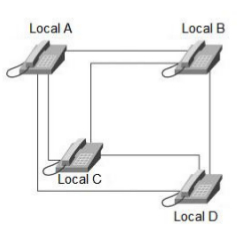
\includegraphics[width=6.0cm]{imagens/rebeBasicaQuatroTel.jpg}
	\caption{Conexão física entre quatro aparelhos telefônicos.}
    \label{Figura1}
    Fonte: \cite{davidson2008}
\end{figure}

Nos dias de hoje esse sistema seria impraticável, pois seria necessário conectar um fio telefônico a cada aparelho telefônico para o qual se desejasse efetuar uma ligação telefônica. Como exemplo da figura \ref{Figura2}, onde existisse apenas oito aparelhos telefônicos, seria necessário no meio físico vinte e oito cabos diferentes, e em cada aparelho sete conexões diferentes \cite{eduardomaronasmonks2006}.

\begin{figure}[h]
	\centering
	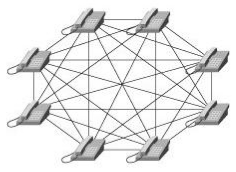
\includegraphics[width=6.0cm]{imagens/rebeBasicaOitoTel.jpg}
	\caption{Conexão física entre oito aparelhos telefônicos.}
    \label{Figura2}
    Fonte: \cite{davidson2008}
\end{figure}

O processo era custoso e havia pouca escalabilidade da estratégia e isto impossibilitou de imediato a expansão do sistema telefônico, mas com o passar do tempo houve a expansão com uso de comutadores (\textit{switches}), onde o sistema de telefonia na necessitava mais de uma ligação física direta entre todos os aparelhos telefônicos dos usuários \cite{thiagowinkler2007}.

Os comutadores realizam a conexão de um usuário através de um único cabo até o escritório central, e de início os comutadores eram pessoas, ou seja, um operador que perguntava qual destino o usuário gostariam se comunicar, e então o operador realizava a manualmente a conexão entre os dois trajetos de voz, a figura 3 exemplifica com fica um operador centralizado para comutar as chamadas entre quatro usuários \cite{eduardomaronasmonks2006}.

\begin{figure}[h]
	\centering
	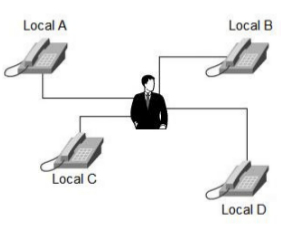
\includegraphics[width=7.0cm]{imagens/operadorCentralizado.jpg}
	\caption{Comutador Humano: Operador Centralizado.}
    \label{Figura3}
    Fonte: \cite{davidson2008}
\end{figure}

Os comutadores começaram a se tornarem automáticos, surgindo então o conceito de discagem para encontrar o destino das ligações, pois o números de ligações já estavam com grande volume, e conceito de comutadores manuais já estava impraticável. Os comutadores evoluirão de manuais, para eletromecânicos e consequentemente para eletrônicos com enorme capacidade de processamento. Através de técnicas de amplificação de sinal, bem como a automatização, digitalização e a escalabilidade necessária os serviços de telefonia permitiram a comunicação ao redor do mundo, com grande expansão. As duas formas de transmissão de voz na telefonia e a forma analógica e a forma digital. \cite{books/daglib/0018909}.

Por diversas décadas o sistema de telefonia permaneceu na estrutura analógica de transmissão, pois todo o som que se houve, inclusive o voz humana está no formato analógico. Em um sistema de telefonia de curto alcance, ou seja, de usuário próximo a central telefônica fazendo a ligação com outro usuário não era problema, porém com distancias cada vez maiores foi necessário a amplificação dos sinais de voz, mas devido a comunicação analógica os ruídos também são amplificados, ou seja, eram intensificados. Com relação aos PABX (\textit{Private Automatic Branch Exchange}), os ramais em sua maioria são analógicos com poucas exceções digitais dependendo dos recursos da central \cite{books/daglib/0018909}.

A solução empregada foi de regenerar os sinais em vez de amplificá-los, porém só é possível, por um processo de amostragem e quantização da amplitude dos sinais analógicos durante determinado período de tempo, ou seja,  por meio da sua digitalização, que transformam esses sinais em 0 (zeros) e 1 (uns) e posteriormente transmiti-los \cite{alexandrekeller2014}.

Para suprir a deficiência da transmissão analógica, surgiu então a transmissão digital, esta ainda permitiu que a voz fosse transferida em redes de pacotes. A digitalização da voz é realizada através de \textit{codecs} (codificadores/decodificadores) de voz, e sua transmissão e realizada por centrais telefônicas, ou seja, por \textit{backbone} das provedoras de serviços. Os comutadores realizam a conversão analógico/digital quando o sinal for em direção ao assinante. O PCM (\textit{Pulse Code Modelation}) é o \textit{codec} mais utilizado. Segundo \citeonline{gomeslemoscolcher1995}, as técnicas empregadas de amostragem são baseadas no teorema de Nyquist, onde o número de amostras deve ser duas vezes maior, do que a maior frequencia de sinal.

O processo de digitalização de voz usando PCM funciona da seguinte forma \cite{eduardomaronasmonks2006}:

\begin{figure}[h]
	\centering
	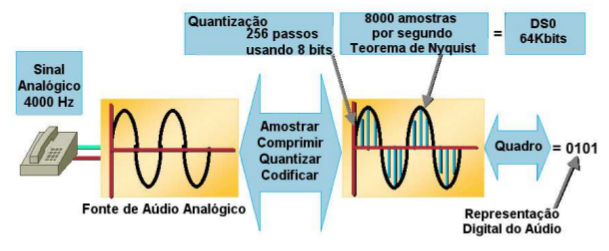
\includegraphics[width=16.0cm]{imagens/processoPCMdigital.jpg}
	\caption{Processo PCM de digitalização de voz.}
    \label{Figura4}
    Fonte: \cite{eduardomaronasmonks2006}
\end{figure}

\begin{itemize}
  \item As formas de ondas analógicas são passadas por um filtro de voz para eliminar qualquer freqüência acima de 4000 Hz. Estas freqüências são filtradas até 4000 Hz para limitar a quantidade de interferência entre linhas (crosstalk) na rede de voz.
  \item É feita a amostragem do sinal analógico na taxa de 8000 vezes por segundo.
  \item Após a amostragem, o sinal é convertido em um formato digital discreto. A amostra é representada por um código que indica a amplitude da forma de onda no instante da amostragem. O PCM utilizado em telefonia usa 8 bits em cada amostra.
\end{itemize}
	
O PCM utiliza largura de banda nas chamadas de 64 Kbps também conhecido como DS-0, sendo que utiliza um código de de 8 bits registrado 8000 vezes por segundo para a codificação dos sinais de áudio, é o equivalente a um circuito de 64 Kbps (8 bits x 8000s) \cite{alexandrekeller2014}.

Existe duas variações de codificações do PCM, o padrão de codificação norte americano e japonês, que é G.711u também conhecido como m-law, e ainda o padrão de codificação europeu e de outros países inclusive o Brasil que é o G.711a também conhecido como a-law, possuem minímas diferenças, onde o m-law tem uma pequena vantagem sobre à performance na sinalização de ruídos de baixo nível \cite{gomeslemoscolcher1995}.

\subsection{Infra-estrutura da PSTN}
O atual sistema de telefonia, também chamado de PSTN (\textit{Public Switch Telephone Network}), foi planejado para acomodar uma única aplicação, ou seja, a voz não comprimida. Estas redes foram construídas para entregar 99,9994$ \% $ das chamadas, com baixa latência, e roteamento de chamadas altamente escalável através da infra-estrutura SS7 (\textit{Signaling System 7}, e serviços de voz de valor agregado como mensagem de voz e identificador de chamadas.

A infraestrutura inicial de telefonia começa com os pares de fios conectados ao terminal telefônico, chamado local loop, estes pares de fios são conectados a uma central telefônica, seja ela uma central particular como um PABX ou um provedor de serviços de telefonia. O tronco (\textit{trunk}) é a comunicação entre comutadores centrais ou entre PABXs. \cite{eduardotude2014}.

\subsubsection{Tipos de sinalização e estabelecimento de circuitos}
A sinalização é realizada em dois sentidos, usuário/rede telefônica e rede telefônica/rede telefônica. A primeira situação é a forma de como usuário final se comunica com a rede telefônica, geralmente através de um um terminal analógico. O DTMF (\textit{Dual Tone Multi-Frequency}) é o método mais comum, e possibilita através da variação da frequência representar dígitos e comandos no terminal telefônico, sua transmissão ocorre no mesmo caminho da voz, conhecido como sinalização inband \cite{thiagowinkler2007}.

Existem protocolos de sinalização inband e outband. Os protocolos inband entre centrais foram abolidos nos anos 70, por limitações técnicas e por serem susceptíveis a fraudes. O protocolo outband possui um caminho independente da voz, como o protocolo SS7 (\textit{Signaling System 7}), este protocolo  reserva um canal de 64kbits para controle das chamadas e através de pacotes controla as conexões na central e entre centrais, permite ainda funções como identificação do telefone chamador e diminuição no tempo de complemento de chamadas, atualmente e protocolo padrão \cite{eduardomaronasmonks2006}.

As especificações dos sinais elétricos indicam se o circuito e circuito do tipo E1 ou T1, ou seja, a rede telefônica poder ser vista como uma malha de cabos e sinais elétricos, onde a especificações das variações dos sinais elétricos indica os eventos e ocorrências de cada circuito. Tanto no Estados Unidos como no Japão utilizam-se circuitos DS-0 de 24 grupos, os chamados T1, que fazem uso do codec m-law e ocupam 1544 Mbps, 24 canais de 64 Kbps, mais 8 Kpbs utilizados na sinalização dos frames de dados. Já na Europa e nos demais países utiliza DS-0 de 32 grupos, os chamados de E1, utilizando o codec a-law, sendo 30 canais de 64 Kbps para trafegar voz, 1 canal para sinalização e 1 para sincronia do link de comunicação, totalizando 2048 Mbps \cite{alexandrekeller2014}.

Os circuitos E1 que utilizam TDM (\textit{Time-Division Multiplexing}), são constituídos de canais fixos de voz, sinalização e sincronia, ou seja, o canal zero é sempre o canal de sincronia, o canal dezesseis e sempre o canal de sinalização, e são conhecidos como canais D (delta), e os demais canais B (Bearer), onde definitivamente trafega o áudio das chamadas, é exemplifica na figura \ref{Figura5} \cite{andersonramires2005}.

\begin{figure}[h]
	\centering
	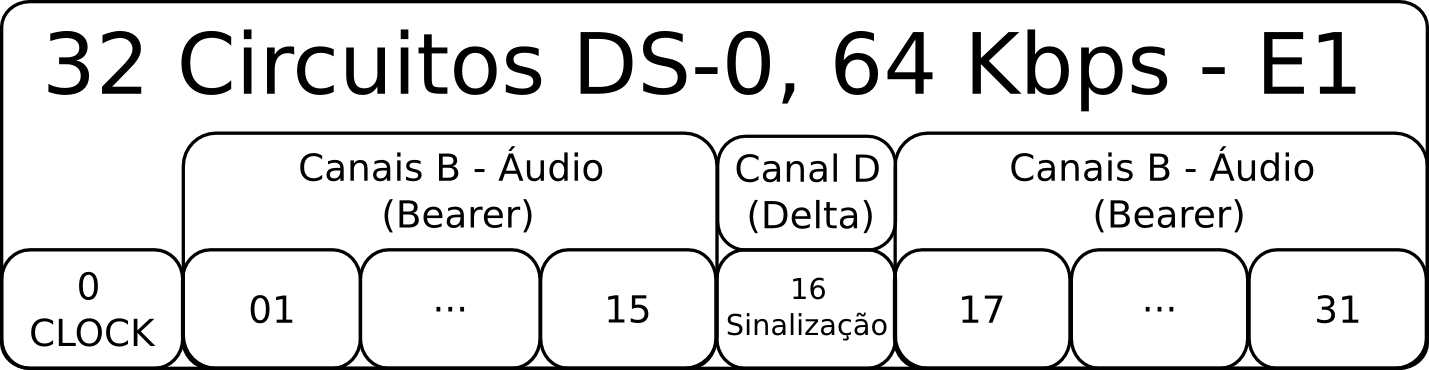
\includegraphics[width=15.0cm]{imagens/LinkE1.png}
	\caption{Diagrama de um circuito E1.}
    \label{Figura5}
    Fonte: \cite{alexandrekeller2014}
\end{figure}

\subsubsection{Estabelecimento de um circuito, ou chamada telefônica}

Não é apenas áudio que trafega durante uma chamada telefônica, ocorre uma série de trocas de sinais entre o originador da chamada e recebedor, onde a correta transmissão e a identificação desses sinais influenciam diretamente no correto estabelecimento e encerramento da chamada, pois um usuário A deseja se conectar a um usuário B, o usuário a retira do gancho o fone (\textit{off-hook}), e logo o equipamento a qual o telefone esta conectado emite um um sinal sonoro, ou seja, tom de discagem (\textit{dial tone}), isto avisa ao usuário que já pode digitar os dígitos referentes ao número de telefone do usuário B, o envio destes digitos até a operadora é realizado por DTMF (\textit{Dual-Tone Multri Frequency}), que a representação sonoro dos números 0 à 9 mais os sinais \# (\textit{sustenido}) e $ \ast $ (\textit{asterisco}) \cite{alexandrekeller2014}.

Cada país possui tons específicos de DTMF, e a operadora a identificar o termino dos envios dos dígitos, emiti um sinal de chamando (\textit{ringing}) para o usuário A, e ao usuário B atender, emite a operadora um sinal de (\textit{off-hook}), então o circuito é fechado, e a comunicação é estabelecida. A partir deste momento o som produzido pelo participantes da chamada é transmitido até que um dos usuários termine a conexão, colocando de volta o fone no guancho (\textit{on-hook}), gerando um sinal de desligamento (\textit{hangup}) para operadora, liberando assim o circuito que havia sido gerado \cite{eduardotude2014}.

Mas liberação desse circuito depende do lado de quem finalize a chamada, conforme normas brasileiras, se originador da chamada é o usuário A, os custos da chamada pertence a ele, então se ele finalizar a chamada, ela será finalizada de imediato, caso seja o usuário B, recebedor da chamada, a chamada continuara ativa por 90 segundos, pois que tem o direito de encerrar o circuito e só originador da chamada, porém se a chamada originar do usuário A, mas com cobrança direcionado ao usuário B, também conhecidas como “ligações a cobrar” o direito da desconexão passa para o usuário B \cite{andersonramires2005}.

O DTMF é amplamente utilizado em circuitos analógicos, mas existem outros dois digitais amplamente utilizados, que utilizam a sinalização CAS (\textit{Channel Associated Signalling}), sendo eles o MFC e o R2-Digital, ainda há a RDSI (\textit{Rede Digital de Serviços Integrada}), ou no inglês ISDN (\textit{Integrated Service Digital Network}), que utiliza a sinalização CCS (\textit{Commom Channel Signalling}) \cite{alexandrekeller2014}.

\subsubsubsection{Sinalização multi-frequency}
A sinalização MF (\textit{multi-frequency}) ou multifrequencial, utiliza de tons para permitir a troca de sinalização envolvida para o estabelecimento de uma chamada, já a sinalização MFC/R2-Digital, utiliza o MFC (\textit{Multi-Frequency Code}), pois a sinalização entre dois pontos depende de uma sequencia preestabelecida. Getalmente essa troca de sinalização ocorre da seguinte forma: \cite{davidson2008}

\begin{itemize}
  \item A envia um sinal multifrequencial e o mantém até que B o receba e confirme.
  \item O usuário B confirma o recebimento com outro sinal multifrequencial, essa confirmação também significa uma solicitação para A, e B mantém o sinal multifrequencial durante o processo.
  \item A percebe que B confirmou o recebimento do sinal multifrequencial e retira o sinal multifrequencial que o enviou, assim dependendo de que B solicitar A fica pronto para o envio de um novo sinal multifrequencial.
  \item B percebe que A retirou o sinal multifrequencial, e também retina seu sinal multifrequencial, e B fica apto a receber uma nova solicitação de A. O ciclo repete até o termino da troca de sinalizações entre os terminais de A e B envolvidos na chamada.
\end{itemize}

\subsubsubsection{Sinalização R2-Digital}

O padrão brasileiro de sinalização para links digitais de telefonia no padrão E1 é o R2-Digital comumente conhecido, por utilizar do CAS (\textit{Channel Associated Singalling}), ou simplesmente sinalização associada ao canal, acaba se tornando lento e inflexível. O CAS possui três grupos de sinais: \cite{thiagowinkler2007}

\begin{itemize}
  \item \textbf{Sinais de supervisão}, representam os eventos que ocorrem durante uma chamada e geralmente são específicos para cada variação do CAS de cada região ou país. São também chamados de sinais de linha (\textit{line signals}), e incluem requisição do canal (\textit{seizure}), wink e answer (\textit{atendimento}). No Brasil utilizamos  também o termo “sinalização de linha” para esses sinais, que estão associados ao canal dezesseis e representam os sinais de R2.
  \item \textbf{Sinais de endereçamento}, é o numero de destino, ou seja, os números enviados, são específicos para as variações do CAS implementadas em determinada região, utilizam como base a sinalização multifrequencial. Os tons multifrequenciais são utilizados para transmitir o ANI (\textit{Automatic Idendification Number}), conhecido de forma vulgar como DNIS (\textit{Dialed Number Identification Service}), ou simplesmente \textit{Caller ID}, que não verdade significa que são enviados o número de destino e categoria do originador da chamada. Esses sinais são conhecidos como sinalização de registro no Brasil, pois utiliza sinal multifrequencial através do canal D (\textit{delta}) para envio da sinalização de registro, onde corresponde ao circuito que será utilizado após a chamada ser completada, assim podemos dizer que a sinalização é associada ao canal, ou seja, ao CAS.
  \item \textbf{Tons de anúncios}, são os tons de ringing (\textit{chamando}), ocupado (\textit{busy}), ou mesmo anúncios de “\textit{o número chamado não existe}.
\end{itemize}

A sinalização MFC/R2-Digital trata de forma única e exclusivamente de sinais de áudio, ou seja, tons para identificação da troca sinalização, onde o sinal multifrequencial e enviado dentro do próprio canal de áudio e os sinais de supervisão R2 da chamada dentro do canal dezesseis, específico para essa finalidade. E a conversão dos sons para o meio digital exige grande poder de processamento \cite{davidson2008}.

\subsubsubsection{Sinalização ISDN}
O RDSI ou ISDN, foi concebido em meados dos anos 1980, é o modelo de sinalização para circuitos de telefonia TDM, considera-se como a evolução natural do MFC/R2, pois além de trafegar áudio, ele trafega também todos os tipos de informação, como mensagens de texto, e até mesmo video. Utiliza um canal único para a sinalização da chamada, o CCS (\textit{Commom Chanel Signalling}), mais precisamente o canal dezesseis do circuito, através de pacotes de dados no formato Q.931. O Q.931 controla as requisições e respostas às mensagens de setup da chamada, o reconhecimento do setup, progresso da chamada, mensagens de alerta, desconexão (desligamento) e de informações \cite{alexandrekeller2014}.

O Brasil adotou o EUROISDN como padrão de configuração para ISDN, porém existe outros modelos como o 4ESS, 5ESS, NI1 e Q.Sig. Um circuito E1 ISDN é conhecido como PRI (\textit{Primary Rate Interface}), ou ainda, 30B+D, em referencia aos trinta canais de dados (B – \textit{Bearer}), e um canal de sinalização (D – \textit{Data}).

O ISDN é extremamente rápido e flexível comparado ao MFC/R2, e é semelhante o protocolo TCP/IP usando pacotes de dados para transportar as informações. Mas ainda existem localidades no Brasil onde as centrais telefônicas são antigas e não houve investimento em atualização tecnológicas por parte das operadoras de telefonia, principalmente nas regiões Norte, Nordeste e Centro-Oeste e nestas localidades só tem disponível a sinalização MFC/R2 \cite{eduardotude2014}.

\subsubsection{Termos referentes a Links E1}
Alguns termos utilizados quando nos referimos a links E1, seja com sinalização MFC/R2 ou com ISDN: \cite{alexandrekeller2014}

\begin{itemize}
  \item \textbf{Alinhamento}, o link E1 deve sempre alinhando, ou seja, o canal de comunicação 1 (um) de lado do circuito deve estar alinhado com o canal 1 (um) do outro lado do circuito. O alinhamento e estabelecido pelo lado do circuito configurado como originado do clock, ou seja, é o lado que vai estabelecer o início do alinhamento dos 30 canais de comunicação do link E1.
  \item \textbf{Escorregamento}, é a perda do alinhamento entre os canais, em decorrência da perda de sincronia do clock, onde por exemplo o canal 10 (dez) de um lado não esta mais alinhado com o canal 10 do outro lado do circuito.
  \item \textbf{TAPS}, é o cancelamento do eco, ou mesmo supressores de eco, onde após realizarem a identificação e o treinamento (echotraining) do nível do eco dentro da ligação, aplicam os filtros ao áudio da chamada dependendo do valor do TAPS, como 32 TAPS (4 ms), 64 TAPS (8 ms), 128 TAPS (16 ms ), 256 TAPS (32 ms) e 512 TAPS (64 ms).
\end{itemize}

\section{Voz sobre IP (VoIP)} %\label{cap_exemplos}
%\thispagestyle{empty}
\subsection{Funcionamento do VoIP}
Desde o ano de 1962 a transmissão de voz através da rede de computadores vem sendo arquitetada, em 1977 foi proposto um protocolo para a transmissão de voz em forma de pacotes para uso militar, pelo IETF (\textit{Internet Engineering Task Force}) através de uma RFC (\textit{Request for Comments}) \cite{dancohen1977}.

A tecnologia de VoIP surgiu definitivamente em Israel no ano de 1995, por um grupo de pesquisadores, interessados em desenvolver um sistema que permitisse utilizar os recursos multimídias de um computador doméstico para iniciar o trafego de voz digitalizada através da internet. No ano seguinte o ITU (\textit{International Telecommunication Union}) disponibilizou a primeira versão da recomendação H.323, sendo considerado o primeiro padrão para VoIP \cite{eduardomaronasmonks2006}.

Uma série de técnicas e protocolos são utilizados para transportar a voz em uma rede de pacotes. Os codecs  codificadores/decodificadores, fazem a transformação das ondas sonoras da voz em  códigos binários, ou seja, assim que a voz e captada pelo microfone as amostras passam pelos processos de quantização, codificação e compressão, para que possa ser transportada de maneira eficiente em rede de pacotes, como demonstrado na figura \ref{Figura6}. Após sua compressão o fluxo de bits é encapsulado em datagramas UDP, e posteriormente encapsulado em pacotes IP, logo os pacotes são transportados sem qualquer distinção pela rede, como qualquer outro pacote de dados. No receptor é que acontece o processo de descompressão, decodificação da voz, porém este tem que possuir o codec apropriado \cite{eduardomaronasmonks2006}.

\begin{figure}[h]
	\centering
	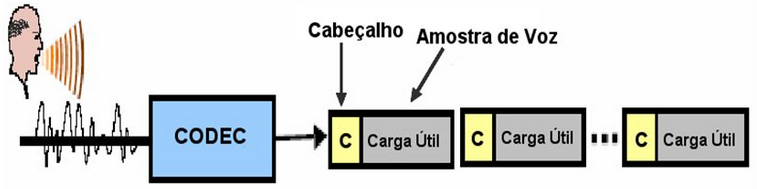
\includegraphics[width=15.0cm]{imagens/transmissaoVozRde.jpg}
	\caption{Transmissão da voz através de rede de pacotes.}
    \label{Figura6}
    Fonte: \cite{eduardomaronasmonks2006}
\end{figure}

O Funcionamento do VoIP ocorre através de comutação de pacotes e para que os pacotes sejam enviados faz-se, necessário, o perfeito funcionamento dos protocolos. O protocolo é o padrão para a comunicação de dados e na interligação de redes, a rede não funciona sem os protocolos, um protocolo é que especifica como um programa deve preparar os pacotes para serem enviados para o próximo estágio no processo de comunicação. \cite{andersonramires2005}.

\subsection{Tipos de Redes}
O VoIP pode utilizar tanto redes baseadas em circuitos, onde é a forma  tradicional de rede para carregar a voz, como rede baseadas em pacotes, que conecta e transporta informações entre computadores remotos.

\subsubsection{Redes baseadas em circuitos}
A comutação de circuito é a tecnologia tradicional de rede empregada para carregar a voz, é orientada a conexão, utiliza técnicas de multiplexação para concentrar inúmeras conversações em um único tronco físico. A TDM (\textit{Time Divison Multiplexing}) é uma técnica de multiplicação que não utiliza de funções complexas de controle de tráfego. Os usuários não podem afetar a qualidade de serviços um do outro, e são assinalados a intervalos de tempo fixo, consequentemente a qualidade do serviço é determinística e previsível. O TDM não permite maximizar a utilização de banda utilizada, e transferências como de arquivos e video conferencia necessitam de banda variável em suas transmissões, o TDM aloca fatias de tempo para uma conexão mesmo se o usuário não estiver transmitindo algo, como obeservado na figura \ref{Figura7}, isso garante a qualidade mas desperdiça recursos, se torna ineficiente para tráfego com características de rajada, devido a sua alocação estática. Porém é eficiente
para suportar trafego de voz \cite{thiagowinkler2007}.

\begin{figure}[h]
	\centering
	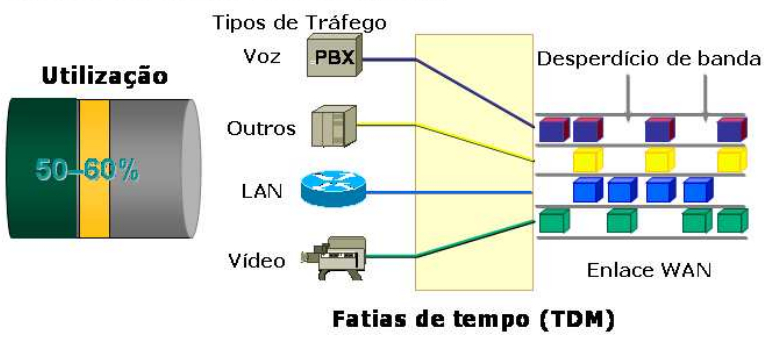
\includegraphics[width=16.0cm]{imagens/comutacaoCircuitosTDM.jpg}
	\caption{Comutação de Circuitos (TDM).}
    \label{Figura7}
    Fonte: \cite{eduardomaronasmonks2006}
\end{figure}

\subsubsection{Redes baseadas em pacotes}
Transportar informações entre computadores remotos é a finalidade da rede de comunicação de dados. Sua eficiência se da por transmitir o mais rápido possível a maior quantidade de informações válidas entre o máximo de usuários. A vazão (throughput) medida em bits por segundo, é que determina o desempenho básico em rede de computadores. Os congestionamentos que geralmente causam o aumente de retransmissão das informações e as perdas de pacotes, em consequência disso acaba afetando a vazão \cite{davidson2008}.

Os usuários acabam percebendo a variação de sobrecarga da rede, através do aumento de tempo de resposta, ocasionando insatisfação sobre a qualidade do serviço prestado. O comportamento transparente seria o ideal, pois para os usuários e como eles estivessem interligados sem o compartilhamento de recursos, assim não haveria nenhum tipo de contenção de tráfego causado pela rede. A comutação de pacotes é a tecnologia tradicional de rede para carregar dados, os pacotes podem ser comutados sem estabelecer uma conexão previa. O protocolo IP é um exemplo, pois os pacotes são roteados em cada nó da rede e nenhuma banda é pré-alocada para a transferência de dados. Esta tecnologia maximiza o uso da rede, porém não garante a qualidade de serviço pois, não há qualquer alocação de recursos, obeservado na figura \ref{Figura8}. A largura de banda ocupada pelo usuário acaba variando a cada instante de acordo com a carga da rede, onde esta tem a característica de rede de melhor esforço (\textit{best
effort}) \cite{adrianoramosgoncalves2001}.

Outros exemplos de redes baseados em pacote são a IPX(\textit{Internet Packet Exchange}), MAN (\textit{Redes Metropolitanas}), as WAN (\textit{Wide Area Network}) que são as redes de longa distância e ainda conexões discadas usando PPP (\textit{Point-to-Point Protocol}).

\begin{figure}[h]
	\centering
	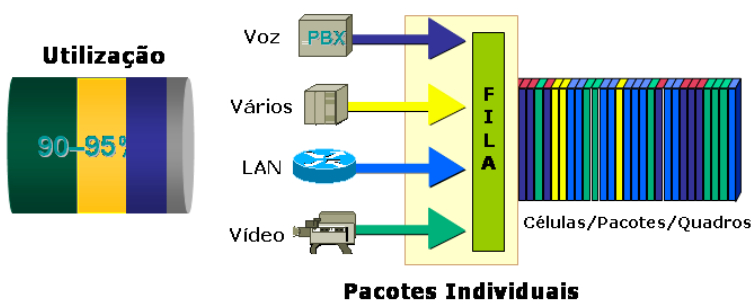
\includegraphics[width=16.0cm]{imagens/comutacaoPacotes1.jpg}
	\caption{Comutação de Pacotes.}
    \label{Figura8}
    Fonte: \cite{eduardomaronasmonks2006}
\end{figure}

\subsection{Protocolos}

Os protocolos VoIP podem ser categorizados como protocolos de sinalização e  protocolos de mídia. Basicamente existe protocolos de sinalização proprietários e abertos em VoIP, entre os proprietários estão o Skynny da Cisco, utilizado no serviço Skype e as variações dos protocolos abertos, a exemplo do protocolo SIP, que está sendo utilizado no Microsoft Messenger. Apesar de haver uma grande base destes protocolos proprietários, cada vez mais os fabricantes de equipamentos estão adotando os protocolos de padrão aberto, principalmente o SIP. Entre os protocolos de sinalização abertos os mais utilizados são: \cite{davidson2008}
\begin{itemize}
  \item H.323 (\textit{Sistemas Audiovisuais e Multimídia});
  \item SIP (\textit{Session Initiation Protocol});
  \item MGCP (\textit{Media Gateway Control Protocol});
  \item IAX (\textit{Inter-Asterisk Exchange}).
\end{itemize}

Há ainda os protocolos responsaveis pelo tráfego da mídia são o RTP (\textit{Real Time Protocol}) e o protocolo auxiliar RTPC (\textit{Real Time Control Protocol}). Ambos são transportados sobre os protocolos UDP e IP \cite{davidson2008}.

\subsubsection{Protocolos de sinalização}

\subsubsubsection{Protocolo H.323}
O H.323 é o protocolo mais aproveitado em sistemas de comunicação multimídia baseado em pacotes. Faz parte da família de recomendações ITU-T (\textit{International Telecommunication Union Telecommunication Standardization Sector}) H.32x, a qual pertence à série H da ITU-T, versando sobre “Sistemas Audiovisuais e Multimídia”. O padrão H.323 tem como objetivo especificar sistemas de comunicação multimídia em redes baseadas em pacotes, que não fornecem QoS (\textit{Quality of Service}) garantida. Ainda estabelece padrões tanto de codificação como descodificação de fluxos de dados de áudio e vídeo, garantindo que um fabricante que utiliza o padrão H.323 em seu produto interopere com produtos de outro fabricante que também utilize o H.323 \cite{thiagowinkler2007}.

Em relação a aspectos relacionados a rede o padrão H.323 é completamente independente, logo pode ser utilizado em quaisquer  tecnologias de enlace, podendo optar tanto pelas lideres do marcado atual como a Ethernet, Fast Ethernet, FDDI (\textit{Fiber Distributed Data Interface}) ou mesmo a Tonken Ring. Ainda não possui qualquer tipo de restrição quanto a topologia da rede, podendo forma-se a uma ligação única ponto a ponto, ou um único segmento de rede, ou ainda serem complexas, envolvendo vários segmentos de rede \cite{eduardomaronasmonks2006}.

O padrão H.323 especifica o uso de  áudio, video e de dados em comunicação, porém apenas o suporte a mídia de áudio é obrigatório, e cada mídia (áudio, vídeo e/ou dados), quando utilizada deve seguir as especificações do padrão. Pode-se ter uma variedade de formas de comunicação, como envolvendo apenas áudio, áudio e video, áudio e dados, ou áudio, vídeo e dados \cite{glauciadasilvaribeiro2011}.

\subsubsubsection{Protocolo SIP}
O SIP (\textit{Session Initiation Protocol}), é um protocolo de aplicação baseado em texto, padrão da IETF (\textit{Internet Engineering Task Force}) RFC 3261 (\textit{Request for Comments}), similar ao HTTP (\textit{Hyper Text Transfer Protocol}) que utiliza o modelo requisição/resposta, para iniciar sessões de comunicação interativa entre usuários. O protocolo SIP é utilizado para estabelecer chamadas e conferencias através de redes via IP. Uma chamada pode usar diferentes tipos de dados, incluindo áudio, vídeo e muitos outros formatos, ou seja, a configuração da sessão, mudança ou término é independente do tipo de mídia ou aplicação que é utilizada em uma chamada \cite{adrianoramosgoncalves2001}.

A origem do protocolo SIP teve origem no ano de 1996, logo após o protocolo H.323 ser finalizado como padrão, porém o SIP teve uma rápida adoção como padrão para comunicações integradas e aplicações que usam presença\footnote{Presença significa a aplicação estar consciente da sua localização e disponibilidade}. O SIP levas os controles da aplicação para o terminal, eliminando a necessidade de uma central de troca.

O SIP ao estabelecer ou terminar uma comunicação possui cinco passos básicos:
\begin{itemize}
  \item \textbf{Localização do Usuário,} determinar a localização do usuário na rede. Os usuários podem se mover para outros locais e acessar o seu telefone e uncionalidades de aplicações remotamente. Por exemplo, em uma rede corporativa o usuário receberá chamadas para o seu ramal não importando onde esteja dentro da empresa.
  \item \textbf{Disponibilidade do Usuário,} verifica se o usuário deseja ou está, disponível para comunicação.
  \item \textbf{Capacidade do Usuário,} determina os parâmetros e o formato da mídia a serem usados na sessão. A negociação dependerá da capacidade dos equipamentos envolvidos.
  \item \textbf{Configuração da Sessão,} chamadas ponto a ponto ou em conferência devem ser estabelecidas, com os parâmetros negociados.
  \item \textbf{Gerenciamento da Sessão,} incluem-se neste a transferência e terminação de sessões, a modificação de parâmetros da sessão e o carregamento de novos serviços.
\end{itemize}

O SIP é utilizado sobre o protocolo UDP por razões de desempenho, porém providencia seus próprios mecanismos de garantia de entrega. Caso necessário as mensagens SIP podem ser utilizadas de forma criptografadas sobre o protocolo TLS (\textit{Transport Layer Security}) ou através de tunelamento, com VPN (\textit{Virtual Private Network}) \cite{davidson2008}.

A VPN ainda pode solucionar o problema do SIP quando há o emprego de NAT (Network Address Translator) em qualquer um dos lados, ou seja, tanto na rede do originador como do receptor da chamada, pois o SIP armazena os endereços de origem e destino dentro do campo de dados dos pacotes TCP/IP, já o NAT trata os endereços armazenados dentro da camada de rede dos pacotes. Logo a informação não é atualizada e, assim, os pacotes não contem os endereços corretos para a entrega dos pacotes aos cliente envolvidos \cite{alexandrekeller2014}.

\subsubsubsection{Protocolo MGCP}
O protocolo MCGP (\textit{Media Gateway Control Protocol}) do IETF teve como objetivo a integração da arquitetura SS7 (\textit{Signaling System 7}), onde esta é adotada em redes de sinalização na telefonia convencional, com redes IP, Frame Relay e ATM (\textit{Asynchronous Transfer Mode}) \cite{theodorewallingford2005}.

A evolução do MCGP, é um trabalho em conjunto dos grupos do ITU-T e IETF, que resultou na recomendação H.248, também conhecida como Megaco (\textit{Media Gateway Control}), são utilizados nos gateways para controle da mídia e para permitir que um MGC (\textit{Media Gateway Controller}) controle um MG (\textit{Media Gateway}) \cite{theodorewallingford2005}.

\subsubsubsection{Protocolo IAX}
O IAX (\textit{Inter-Asterisk eXchange}), foi criado pela Digium, empresa mantedora do Asterisk, com o objetivo permitir a comunicação entre servidores Asterisk, é um protocolo aberto e já está na sua segunda versão o IAX2. A RFC publicou a sua padronização e homologação que é a RCF5456. É um protocolo que transporta a sinalização e mídia em uma única porta UDP/IP, a 4569, sendo sua configuração bem mais simples em comparação a outros protocolos, como SIP, H.323 e MCGP, especialmente quando a comunicação envolve NAT e ou Firewalls\footnote{Firewall é uma solução de segurança baseada em hardware ou software}. O IAX realmente não tem nenhuma dificuldade para a sinalização e transporte da mídia entre os pontos da conexão, e não faz uso de qualquer outro protocolo para resolver tais dificuldades \cite{alexandrekeller2014}.

O IAX pode trafegar as informação também em modo trunk, que é a multiplexação dos pacotes de dados, ou seja, o áudio de várias chamadas é agrupado em um único conjunto de pacotes, em um único cabeçalho IP, reduzindo a latência, e ainda produzindo uma economia da utilização de banda da rede, pode ainda, utilizar de encriptação das chamadas utilizando chaves simetricas AES (\textit{Advanced Encryption Standart}), ou modo de autenticação com base em chaves criptografadas assimétricas, utilizando RSA (\textit{Rivest, Shamir e Adleman}).\cite{alexandrekeller2014}.

\subsubsection{Protocolos de mídia}

\subsubsubsection{Protocolo RTP}
O protocolo RTP (\textit{Real-Time Transport Protocol}) é utilizado em redes fim a fim, adequado a  aplicações de tempo real, tais como áudio e video, sobre serviços de rede unicast ou multcast. O RTP define como é realizada a fragmentação do fluxo de dados, e a cada fragmento e adicionado informação de sequencia e de tempo de entrega, por utilizar o protocolo UDP, não garante a que os pacotes serão entregues num determinado intervalo, sua homologação é definida pelo RFC3550 \cite{henningcasnervan1996}.

\subsubsubsection{Protocolo RTCP}
O protocolo RTCP é baseado no envio periódico de pacotes de controle a todos os participantes da chamada, utilizando o mesmo mecanismo de distribuição dos pacotes de mídias. Os dados são transmitidos através de um controle mínimo, pois a transmissão acaba ocorrendo em tempo real usando o suporte dos pacotes UDP da rede IP, é um protocolo opcional, pois tem como função a transmissão periódica de pacotes de controle entre os participantes de uma conversação, com objetivo de verificar a qualidade do serviço e transporta informações úteis de tais participantes, é muito utilizado em aplicações de videoconferência \cite{henningcasnervan1996}.

\subsection{\textit{Codecs} (Codificadores e Decodificadores)}
Um codec é um algoritmo que faz a digitalização e a quantificação do sinal áudio e vídeo reduzindo o número de bytes gerados, logo diminui a banda necessária para a transmissão, e por ser digital é uma vantagem para transmissões em curtas e longas distancias, pois, mesmo sofrendo atenuação, perdas inerentes ao meio de propagação, e ação de ruídos, o processo de filtragem de ruídos é bem mais simples do que com os sinais analógicos, e antes da amplificação, o sinal é regenerado pelos repetidores \cite{eduardomaronasmonks2006}.

As características dos \textit{codecs} influenciam diretamente na qualidade do áudio da chamada, a exemplo da ocupação de banda do codec G.711 que utiliza 64Kbps de banda, ou seja, que em cada pacote de dados transmitido 64 Kb do pacote de rede estão sendo ocupados apenas com o áudio da chamada, pois o G.711 não necessita de processamento porque não realiza nenhuma compressão de voz. Já o G.729a tem apenas 8Kbps de ocupação de banda, mas é necessário uma grande capacidade de processamento, pois comprime 8 vezes o áudio \cite{alexandrekeller2014}.

A transcodificação é o processo de conversão de um codec em outro, por exemplo, de G.729a para G.711, isto causará o aumento no delay e na latência, logo poderá prejudicar a qualidade do áudio na chamada. O ideal é que todos os ramais do ambiente tenha a mesma implementação do codec \cite{alexandrekeller2014}.

\subsection{Qualidade do áudio em VoIP}
Uma exigência básica no VoIP é a qualidade do serviço, ou seja, chamadas com áudio de qualidade é dependente de fatores considerados críticos, pois o áudio foi digitalizado, comprimido, e dividido em pacotes para ser transmitido de um ponto a outro. Devido a natureza de redes de dados, alguns desses fatores podem ser: \cite{davidson2008}

\begin{itemize}
  \item \textbf{Perda de pacotes} ocorre normalmente dentro dos roteadores que encaminham os pacotes pela rede. Para que uma chamada VoIP não fique prejudicada não devem ocorrer perdas superiosres a 5\%.
  \item \textbf{Delay} é o tempo decorrido desde a emissão do som na origem da chamada até a chegada do destino. Quanto maior o \textit{delay}, maiores as chances de a chamada ter a sua qualidade prejudicada.
  \item \textbf{Latência ou atraso} é o intervalo de tempo em que um pacote sai de sua origem e chega ao seu destino, ou seja, o tempo que leva para viajar dentro da rede, desde a origem até o destino. Cada roteador em média adicionar 10 ms de latência à comunicação, para que a comunicação não seja prejudicada a latência deve ser inferior a 250 ms.
  \item \textbf{Jitter} é a variação de tempo entre as chegadas de pacotes do endereço de origem ao seu destino, é ocasionado pelo excesso de tráfego ou baixa largura de banda, quanto maior a variação de tempo de tráfego dos pacotes, maior é o \textit{jitter}, o \textit{jitter} pode ocasionar distorção do áudio da chamada, e em cados mais extremos até mesmo o cancelamento da chamada.
  \item \textbf{Eco} é o retorno da nossa própria voz, isso ocorre tanto na telefonia convencional como no VoIP, porém, ocorre muito rápido que acaba sendo imperceptível para os usuários, mas fatores como transcodificação de \textit{codecs}, \textit{gateways}, roteadores, \textit{switches}, largura de banda acabando contribuindo para que eco torne perceptível diminuindo a qualidade da chamada.
\end{itemize}

Há um fator positivo que é o QoS (\textit{Quality of Service}), que é um mecanismo de controle utilizado para priorizar diferentes fluxos de dados dentro da rede, com objetivo de garantir um nível de desempenho de uma aplicação ou programa específico, ou seja, organiza e prioriza os pacotes de uma aplicação como os pacotes de voz, minimizando sua perda dentro da rede. Um detalhe importante é que a implementação de QoS não aumentara a velocidade com que os pacotes trafegam, ele apenas os prioriza e organiza \cite{thiagowinkler2007}.

\subsection{Arquiteturas}
Para implementação do VoIP, existe três arquiteturas básicas, como a \textit{ponto a ponto}, que é mais simples delas, onde nesta arquitetura os terminais fazem uso de \textit{softfones}, telefones IP ou clientes de serviços conhecidos, como \textit{Skype} ou \textit{Jabber} onde conectam-se diretamente entre si, como é demonstrado pela figura \ref{Figura9} \cite{thiagowinkler2007}.

\begin{figure}[h]
	\centering
	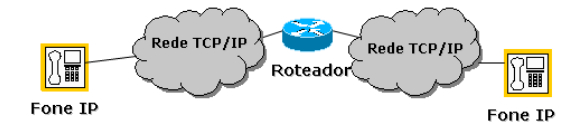
\includegraphics[width=16.0cm]{imagens/pontoaponto.jpg}
	\caption{Arquitetura Ponto a Ponto.}
    \label{Figura9}
    Fonte: \cite{eduardomaronasmonks2006}
\end{figure}

Outra arquitetura é de \textit{gateway}, que integra os serviços de telefonia convencional com a de VoIP, é utilizada para trafegar as ligações através de serviços VoIP sem modificar o serviço de telefonia convencional nos terminais, como demonstrado pela figura \ref{Figura10}. Logo o trafego de ligações entre ligações entre as localidades conectadas com gateways, não será roteado pela rede de telefonia convencional. Essa arquitetura é muito utilizada em empresas ou instituições separadas geograficamente, que aproveitam a estrutura de enlace de dados para fazer o reteamento das chamadas entre as unidades sem passar pela rede de telefonia convencional, economizando no custo das ligações telefônicas \cite{eduardomaronasmonks2006}.

\begin{figure}[h]
	\centering
	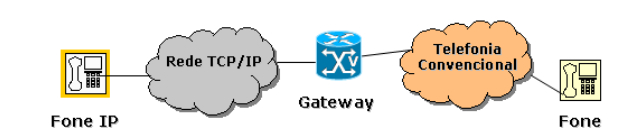
\includegraphics[width=16.0cm]{imagens/gateway.jpg}
	\caption{Arquitetura Gateway.}
    \label{Figura10}
    Fonte: \cite{eduardomaronasmonks2006}
\end{figure}

Por fim, temos a híbrida, que originador da chamada pode estar em uma rede de dados e o destinatário numa rede de telefonia convencional, ou vice-versa, ou mesmo tanto originador como o destinatário numa rede de dados, ou ainda ambos numa rede de telefonia convencional sendo o tráfego transferido através de uma rede de dados como demonstrador pela figura \ref{Figura11}. Portanto, devem haver conversões de codificadores e a numeração deve corresponder a numeração utilizada na rede de telefonia convencional, pois os usuários de VoIP devem originar e receber ligações tanto da rede de dados como da rede telefonia convencional \cite{eduardomaronasmonks2006}.

\begin{figure}[h]
	\centering
	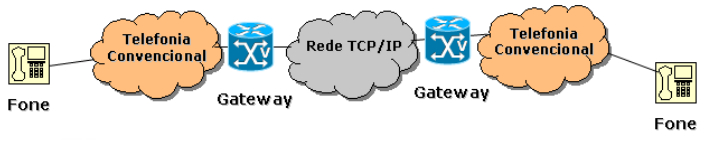
\includegraphics[width=15.0cm]{imagens/hibrida.jpg}
	\caption{Arquitetura Híbrida.}
    \label{Figura11}
    Fonte: \cite{eduardomaronasmonks2006}
\end{figure}

\subsection{Equipamentos}
Terminais, sistemas de controle e gateways são os equipamentos utilizados nas arquiteturas de VoIP. As funções realizadas pelo sistemas de controle recebem diferentes nomenclaturas e diferem em funcionalidades \cite{theodorewallingford2005}.

Os as funções dos terminais se resume em coletar a voz, codificar e transmiti-la. Obedecem a protocolos e recomendações de sinalização de chamadas. Podem ser a nível de \textit{hardware} ou \textit{software}. Os terminais possuem recursos como a configuração de \textit{codecs}, amostras de áudio por pacote, VAD\footnote{Detecta ausência de som em uma chamada, e não transmite esses pacotes de áudio com silêncio pela rede.} (\textit{Voice Activity Detection}) e tamanho de \textit{jitter} \cite{davidson2008}.

Os telefones IP, são exemplo de terminais em \textit{hardware}, existe diversos tipos de telefones IP, que são compatíveis com praticamente todos os protocolos de sinalização, inclusive protocolos proprietários.

Os \textit{softfones}, são exemplos de terminais em \textit{software}, possuim mais funcionalidades que os telefones IP, como maior números de tipos de codecs, maior capacidade de agenda e integração \textit{browsers}\footnote{Browser ou navegador é um programa desenvolvido para permitir a navegação pela internet}, são compatíveis com praticamente todos os protocolos de sinalização, inclusive protocolos proprietários. Interagem com o usuário através de microfone, fones de ouvido e placas de som com capacidade \textit{full-duplex}\footnote{Quando há um dispositivo Transmissor e outro Receptor, sendo que os dois podem transmitir dados simultaneamente em ambos os sentidos}, em uma estação de trabalho (computador), seu custo e bem inferior ao um telefone IP, incluse a \textit{softfones} gratuitos como ekiga \cite{glauciadasilvaribeiro2011}.

As centrais tem a finalidade de controlar e gerenciar as chamadas entre os terminais. Podem ser equipamentos como PABX IP, ou software gratuitos como o Asterisk, que podem ser instalados em um computador o qual pode ser empregado e possuir funcionalidades de PABX IP. Emprega funções de tarifação e distribuição automática de chamadas, políticas de uso, redirecionamento de chamadas, caixa postal, menu interativo e etc. \cite{alexandrekeller2014}.

Os \textit{gateways} ou ATA (\textit{Analog Telephone Adapter)}, tem como função converter a sinalização e mídia das chamadas entre a rede convencional de telefonia e o VoIP, os adaptadores conhecido como ATA, tem a finalidade de de adaptar os telefones analógicos para serem utilizados com VoIP, sendo que a inteligencia da comunicação está inserida no ATA, tendo o telefone como a interface com o usuário \cite{eduardomaronasmonks2006}.


\subsection{Principais benefícios do VoIP}
Uns dos principais benefícios do VoIP é a redução de custo nas chamadas, mais é relativo, pois dependente da quantidade, duração e localidade das chamadas, podendo ser locais, interurbanas ou mesmo, internacionais. Outro fator positivo é infraestrutura única para transportar os dados e a voz,  reduzindo os custos de instalação e manutenção da infraestrutura, bem como, a mobilidade pois o acesso não precisa ser necessariamente em apenas
um único telefone ou computador, e a facilidade de integração com outras aplicações de dados e vídeo \cite{djaneelmajoanine2007}.

\section{Asterisk}
O Asterisk é a implementação de uma central telefônica PBX (\textit{Private Branch eXchange}) em software. Seu nome vem do símbolo (*), muito utilizado na telefonia. Foi desenvolvido por Mark Spencer em dezembro de 1999 e distribuído livremente pela sua empresa \textbf{Digium}, sobre a licença GPL (\textit{GNU General Public License}). Devido a isso, logo obteve um número expressivo de utilizadores e programadores contribuindo para o desenvolvimento da ferramenta, seja testando e reportando eventuais defeitos no sistema ou adicionando novas funcionalidades. Seu desenvolvimento se deu originalmente para o sistema operecional Linux, mas atualmente pode ser instalado e executado em praticamente todos os sistemas operacionais, incluindo o NetBSD, OpenBSD, FreeBSD, Mac OS e até mesmo no Windows. \cite{alexandrekeller2014}

É uma ferramenta que executa todas as funções de uma central telefônica convencional, como URA\footnote{Unidade Respondível Audível.}, correio de voz, salas de conferencia, distribuição automática de chamadas, música em espera, captura, transferência, estacionamento, gravação de chamadas, entre outras, e, caso seja necessário, novas funcionalidades podem ser acrescentadas pelo próprio plano de discagem do Asterisk, módulos customisados escritos em lingugem C ou ainda por meio de \textit{scripts}\footnote{Script é um texto com uma série de instruções escritas para serem seguidas.} escrito em AGI (\textit{Asterisk Gateway Interface}). Outras informações e estastisticas interessantes sobre o Asterisk são: \cite{alexandrekeller2014}

\begin{itemize}
  \item Mais de 1.000.000 de downloads em 2007.
  \item Mais de 1.500.000 de downloads em 2008.
  \item Mais de quatro milhões de servidores instalados e rodando o Asterisk.
  \item Aproximadamente 56.000 fóruns ativos.
  \item Mais de 17.700 lista de discussão sobre o Asterisk.
  \item Aproximadamente 400 colaboradores no projeto.
  \item Mais de 200 provedores de VoIP em todo o mundo utilizando o Asterisk.
\end{itemize}

\subsection{Módulos}
Os módulos que compõem o Asterisk são: \cite{books/daglib/0018909}

\begin{itemize}
  \item \textbf{Asterisk,} contém as funções, aplicações, canais de comunicação e todas as funcionalidades do Asterisk.
  \item \textbf{Asterisk-AddOns,} módulos adicionais ao Asterisk, que não seguem a licença GPL, como funcionalidades de conexão ao servidor MySQL, formato de áudio MP3 e o canal de comunicação com o protocolo H.323. Na a partir da versão 1.8 do Asterisk esses módulos foram incorporados ao pacote principal.
  \item \textbf{Zaptel/DAHDI,} contém os drivers de todas as placas Digium, e de outras fabricantes. Em decorrência de problemas de patente, o nome Zaptel foi renomeado para DAHDI (\textit{Digium Asterisk Hardware Device Interface}), desde agosto de 2008.
  \item \textbf{LibPRI,} biblioteca responsável pela sinalização ISDN/PRI. Necessária sua instalação quando da utilização de uma placa de comunicação digital E1/T1 e sinalização ISDN/PRI.
  \item \textbf{LibSS7,} biblioteca responsável pela sinalização ISUP/SS7. Incorporada ao Asterisk em 2010.
  \item \textbf{LibOpenR2,} biblioteca responsável pela sinalização MFC/R2. Incorporada ao Asterisk em 2010, a partir da versão 1.6.2, pois antes era necessário a utilização de patches\footnote{Patches, são correções ou aumento de funcionalidades de um software (programa de computador).} de correção ao Asterisk para ativar as funções associadas a esse sinalização.
\end{itemize}

\subsubsection{Questões de Hardware}
O Asterisk não possui um DSP (\textit{Digital Signal Processor}) dedicado a cada canal de voz, logo, utiliza o CPU do servidor para processar os canais de voz, fazendo com que o sistema fique muito dependente da performance da CPU, porém, permitiu que o custo fosse reduzido para as placas E1/T1 \cite{flavioeduardoandredade2005}.

Dimensionar e especificar o servidor ideal ao protejo, é problema recorrente até mesmo aos mais experientes consultores de Asterisk, pois precisam avaliar com muita precisão todos os detalhes do ambiente em questão. Porém para que o ambiente seja o mais próximo da realidade possível, é necessário responder algumas questões como: \cite{alexandrekeller2014}

\begin{itemize}
  \item Quantas chamadas simultâneas são previstas para o ambiente?
  \item Haverá gravação das chamadas de entrada e saída?
  \item Haverá a implementação de terminação de chamadas em algum provedor VoIP? Se sim, a quantidade de chamadas simultâneas previstas?
  \item Qual a largura de banda da internet disponível para a comunicação via VoIP com provedores.
\end{itemize}

Os processos que mais consomem processamento é a transcodificação, e a gravação de chamadas em discos. A Digium orienta que, para a transcodificação de 120 chamadas simultâneas entre os codecs G.711 e G729a, é necessário um servidor Intel Xeon 3.0 Ghz com 4 GB de memória RAM. Mas com as questões levantadas, e respondidas de maneira apropriada, pode-se especificar a CPU, sistema de armazenamento de arquivos e a quantidade de memória adequada para o ambiente. \cite{alexandrekeller2014}

\subsubsection{Arquitetura do Asterisk}
O Asterisk é uma ferramente híbrida que executa todas as funções de um PABX, utilizando as principais tecnologias de comunicação existente no mercado, mas em sua arquitetura básica de funcionamento, é necessário quatro componentes, demonstrado pela figura \ref{Figura12}, sendo eles: \cite{books/daglib/0018909}

\begin{itemize}
  \item \textbf{Protocolo,} que realiza á comunicação dos usuários com o servidor Asterisk.
  \item \textbf{Canal de comunicação,} todo cliente possui sua identificação, assim como todo cliente necessita de um protocolo para comunicação, a junção da identificação com o protocolo forma o canal de comunicação.
  \item \textbf{\textit{Codecs},} conversão do sinal analógicos em digital, e posteriormente como é realizado o seu transporte dentro da rede.
  \item \textbf{Aplicaçao,} para conectar as chamadas de entrada com as de saída, ou outros usuários do Asterisk, são utilizadas diversas aplicações como \textit{Dial()} e \textit{VoiceMail()}.
\end{itemize}

\begin{figure}[h]
	\centering
	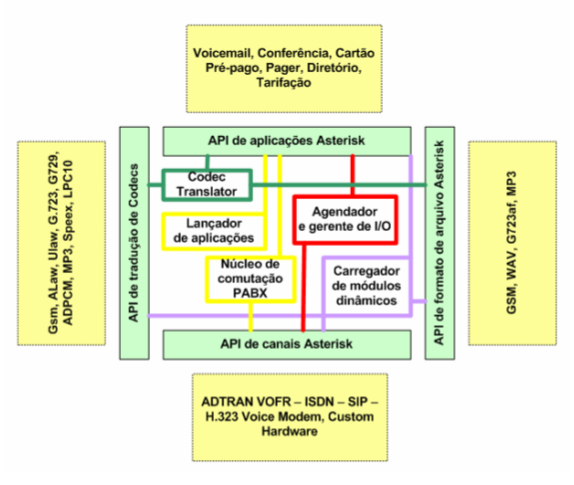
\includegraphics[width=9cm]{imagens/arquiteturaAsterisk.jpg}
	\caption{Arquitetura do Asterisk.}
    \label{Figura12}
    Fonte: \cite{flavioeduardoandredade2005}
\end{figure}

O Asterisk possui funções de PABX de forma integrada, onde um único servidor implementas todas as funções ou em servidores separados, demonstrador pela figura \ref{Figura13}, de acordo com dimensionamento do ambiente em questão. \cite{djaneelmajoanine2007}

\begin{figure}[h]
	\centering
	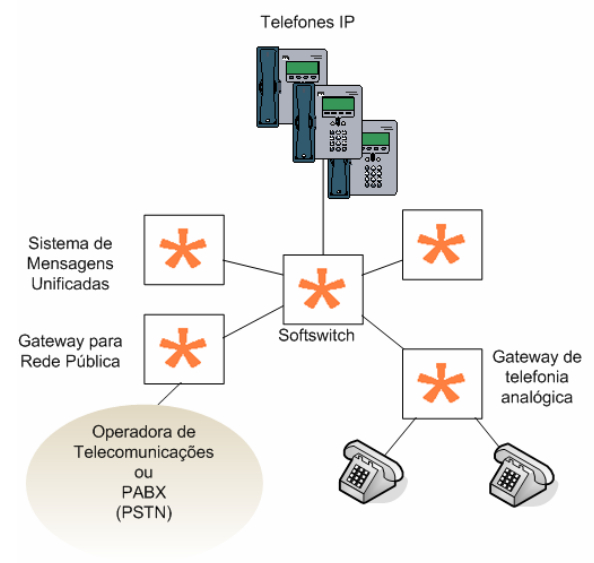
\includegraphics[width=7.5cm]{imagens/servidoresAsterisk.jpg}
	\caption{Múltiplos servidores do Asterisk.}
    \label{Figura13}
    Fonte: \cite{flavioeduardoandredade2005}
\end{figure}

Na figura \ref{Figura14}, é demonstrado um exemplo de PABX de tronco de linha. É um dos sistemas mais simples para empregar o Asterisk. \citeonline{davidson2008} define PABX como, equipamento centralizador de linhas e ramais, também conhecido por central telefônica, que permite a comunicação interna (através de ramais) e facilita  a comunicação externa (linhas telefônicas fixas). 

\begin{figure}[h]
	\centering
	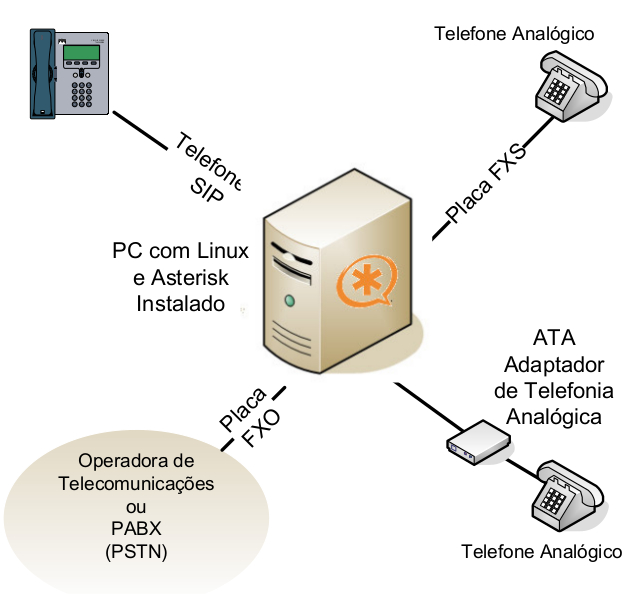
\includegraphics[width=7.5cm]{imagens/PABXAsterisk.jpg}
	\caption{PABX de Tronco.}
    \label{Figura14}
    Fonte: \cite{flavioeduardoandredade2005}
\end{figure}

O PABX poder ser analógico, onde possui circuitos e componentes analógicos, projetados para receber linhas fixas convencionais através das operadoras de telefonia fixa, sua utilização é básica, com alguns recursos como bloqueio de ligações a cobrar e senha nos ramais. Ou pode ser digital, que melhora a qualidade das ligações eliminando ruídos e aumentando o volume do áudio, dispõe de DDR (\textit{Discagem Direta Ramal}) e entrocamento E1. Ou ainda hibrido, onde agrega o melhor das das tecnologias analógica e digital, e implementa a tecnologia VoIP, permitindo interligar filias a custo zero, demonstrado pela figura \ref{Figura15}, reduzindo assim custo, já que depois de configurada ela escolha a rota de menor custo para ligar, dependendo de cada tipo de chamada.

\begin{figure}[h]
	\centering
	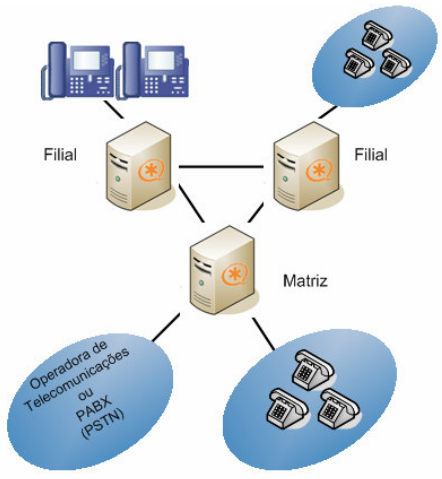
\includegraphics[width=10cm]{imagens/matrizFiliaisAsteirsk.jpg}
	\caption{Interligação de matriz e filiais.}
    \label{Figura15}
    Fonte: \cite{flavioeduardoandredade2005}
\end{figure}




































%%========================= CAPITULO 3 ==============================

\chapter{Falhas e Análise de Requisitos} %\label{cap_exemplos}
%\thispagestyle{empty}
\section{Falhas Apontadas e Obervadas}
Com aplicação do questionário e o com o período de permanecia do teleatendimento da Polícia Militar de Dourados, ficou evidente algumas falhas técnicas e mesmo humanas neste teleatendimento.

\subsection{Aplicação do Questionário}
O questionário foi aplicado com o objetivo de apontar falhas, dentre as questões, a questão \textit{“Você sabe precisar quantas ligações o sistema de telefonia emergencial atende diariamente, e quantas dessas ligação, realmente são ocorrências, e quantas são trotes, pedidos de informação? Se sim informe a quantidade.”}, quatro responderam que sim, porém com valores desencontrados a exemplo o número de ocorrências de um foi 30 já outro foi 70 e assim também foi para os outros questionamentos, percebe que não há como contabilizar a quantidade de atendimentos diários. Outra questão foi \textit{“Você acredita que um sistema de telefonia onde possa gravar e identificar a ligações para este teleatendimento, agregaria vantagens?”}, somente um respondeu que não, pois segundo ele, “A população e hipócrita e mal educada usaria isto em desfavor da PM”, percebe que não como gravar as chamadas, e que por mais que isso seja uma melhoria, na visão deste pode ser maleficio.

\subsection{Falhas Humanas}
Apesar destas falhas não serem objetos de estudo deste trabalho, não deixam de ser um fator preocupante para a eficiência do teleatendimento. E ainda estas falhas acabam relacionando-se indiretamente ou diretamente com algumas falhas técnicas que serão apontadas.

Uma falha verificada foi com relação aos PA (\textit{Pontos de Atendimentos}), ou seja, quando um atendente por algum motivo necessita se ausentar de sua cabine de atendimento e porventura acaba esquecendo de desabilitar o seu PA, isso gera um transtorno para o solicitante pois, a ligação deste solicitante acaba caindo neste PA com o atendente ausente, só que para o solicitante que esta em uma situação urgência, emergência esta sendo gerado tom de chamada, e como consequência ele não é atendido.

Outra falha que coexiste com a anterior, é o fato que o outro atendente tem que se levantar de sua cabine de atendimento, seja para atender a chamada de seu colega de trabalho ou mesmo derrubá-la, ou seja, desabilitar o PA do colega enquanto ocorre uma chamada de um solicitante ou ignorá-la, deixar tocar até dar tom de ocupado para o solicitante.

E os atendentes além de terem que atender as chamadas, ainda tem que ser despachadorores, ou seja, despachar as ocorrências com as viaturas, e nesse momento outra chamada é recebida no PA deste atendente e o mesmo fica impossibilitado de atender esta chamada devido a estar passando as informações da solicitação anterior para a viatura, logo ele ignora ou derruba a chamada.

A ferramenta Asterisk tem funcionalidades técnicas como DAC (\textit{Distribuição Automática de Chamadas}) ou captura de chamadas para amenizar ou mesmo cessar as falhas humanas apresentadas.

A funcionalidade conhecida como DAC ou filas de atendimento, é a maneira que o Asterisk enfileira as chamadas de entrada do servidor, para que posteriormente seja encaminhadas para os agentes de atendimento \cite{flavioeduardoandredade2005}.

Esta funcionalidade geralmente é empregada em \textit{call centers}. E existem dois tipos, os ativos que originam chamadas para o cliente externo oferecendo planos, promoções, etc, e os receptivos, pois trata apenas de chamadas de entrada no sistema, logo o teleatendimento da Polícia Militar se encaixa nesta segunda abordagem. A DAC trás inúmeras vantagens para o teleatendimento, pois organiza as ligações de entrada, e ainda pode-se configurar os atendente para logar-se no servidor PABX, e caso se necessário pode definir um tempo em segundos de inatividade para os atendentes e o próprio servidor coloca este atendente como impossibilitado de atender uma chamada \cite{alexandrekeller2014}.

Captura de chamadas permite que o atendente puxe para seu ramal uma chamada de outro atendente no qual seu ponto de atendimento esta tocando, e pode ser em grupo onde os atendentes pertencem ao mesmo grupo, porém, apenas funciona para canais de comunicação com o mesmo protocolo, ou seja, um canal de comunicação SIP, só pode capturar chamadas de canais de comunicação definidos com SIP. E ainda pode ser direta onde o atendente pode capturar a chamada diretamente discando o número do ramal que se deseja capturar. Esta funcionalidade evita que o atendente tenha que se levantar ou deslocar de sua cabine de atendimento para atender uma PA de outro atendente que esteja tocando \cite{alexandrekeller2014}. 

\subsection{Falhas Técnicas}
As falhas humanas apresentadas, também podem ser consideradas falhas técnicas, pois, no atual momento deste teleatendimento não há nenhuma ferramenta para inibir ou mesmo cessar as falhas identificadas como humanas, porém como demonstrado com as funcionalidades da ferramenta Asterisk podemos saná-las.

A falta de um controle de agentes é uma falha técnica, pois, não há nenhum controle de quando o atendentes ficaram disponíveis para o atendimento das chamadas ou mesmo indisponíveis.

Não existe controle das ligações, ou seja, quantos atendimentos diários foram realizados, quantos desses atendimentos eram realmente ocorrências, quantos eram trotes, pedidos de informação, não há possibilidade do levantamento de estatísticas das ligações recebidas.

Logo não há gravação do áudio das chamadas, isto gera um transtorno tanto para os atendentes como para os cidadãos, pois, caso ocorra uma reclamação contra um atendente, não há como verificar como procedeu o atendimento. E ainda não há uma identificação desta chamadas, mas comumente conhecido como bina, que nada mais é que um serviço telefônico que permite ao assinante chamado identificar o número do terminal originador da chamada.

Outro fator preocupante é a falta da possibilidade de transferência de chamadas, pois, foi verificado que é comum um cidadão retornar a ligação, seja para complementar a solicitação, passar ou repassar algumas informações relevantes para o atendimento, ou mesmo para reportar alguma reclamação, e fica evidente que geralmente o solicitante quer e precisa falar com quem o atendeu anteriormente, e quando este liga novamente acaba sendo atendido por outro. Isso torna-se oneroso pois coleta as informações e repassa posteriormente, ou cede seu PA para o policial anterior complementar as informações, ficando este ocioso.

No teleatendimento, não há uma organização dos ramais, ou seja, não há uma estratégia de atendimento, isto ocasiona uma deficiência com relação ao recebimento das chamadas nos ramais, pois, o primeiro ramal sempre recebera mais ligações do os outros ramais, pelo fato que não há inteligencia no sistema de telefonia, logo se o primeiro ramal estiver desocupado, uma ligação cairá neste ramal, somente quando este estiver ocupado passará para o segundo ramal, isso segue sucessivamente.

Não tem uma padronização no atendimento, ou seja, não há uma mensagem inicial no primeiro contato como uma mensagem de boas vindas para identificar de qual órgão de segurança pública se trata, isto se faz necessário, pois, alguns cidadãos confundem os números emergenciais dos órgãos de segurança públicas.

Os equipamentos utilizados no teleatendimento da Polícia Militar são de uso continuo, e já tem longa data de utilização, e muitos estão apresentando defeitos e avarias, e fica evidente a falta de manutenção ou mesmo a troca devido seu valor elevado.

Assim como nas falhas humanas a ferramenta Asterisk tem funcionalidades como a própria DAC, gravação de chamadas, transferência de chamadas ou teleconferência e bilhetagem para amenizar ou cessar as falhas técnicas deste teleatendimento.

A DAC além de auxiliar nas falhas humanas apresentadas anteriormente, pode auxiliar no controle dos atendentes, pois, estes terão que autenticar-se no sistema para poderem atenderem as chamadas, e com auxilio de outra funcionalidade que é a bilhetagem podemos ter todas informações de autenticação dos usuários, bem como, controle de todas as informações das chamadas, identificação da chamada, tempo médio de espera, tempo médio de atendimento, quantidade chamadas abandonadas, ou seja, aquelas que o cidadão desistiu, e ainda criar estrategias de atendimento para os atendentes, ou seja, a chamada vai cair para o atendente que esta mais tempo sem atender uma chamada, aquele que não concretiza um atendimento, aleatoriamente entre outras \cite{books/daglib/0018909}.

A DAC ainda permite uma padronização do atendimento, pois pode empregar uma URA, com uma mensagem identificando o órgão de segurança pública, e caso tenha pelo menos um atendente disponível transfere a chamada para ele, caso tenha mais de um, utiliza uma das estrategias de atendimento mencionados no paragráfo anterior, e não havendo nenhum, cai direto na fila de atendimento, e pode informar com uma mensagem automatica a posição a qual se encontra na fila, ou seja, quantos estão na sua frente aguardando o atendimento e ou ainda colocar uma musica em espera \cite{flavioeduardoandredade2005}.

Bilhetagem é o armazenamento de todas as informações de todas as chamadas executadas ou recebidas, podem ser simplesmente arquivos de texto simples ou ainda serem armazenados em banco de dados externos como MySQL ou Postgresql através de ODBC (\textit{Open Database Connectivity})\footnote{Padrão aberto de conectividade com praticamente qualquer banco de dados disponível}. Porém bilhetagem não é tarifação, ou seja, cobrança de custos das ligações \cite{alexandrekeller2014}.

A gravação da chamadas podem ser a nível de atendente ou não própria configuração da fila, e ainda pode ser implementada de duas formas, sendo por meio de aplicação onde toda chamada e gravada e não existe a possibilidade de interrompê-la, ou sobre demanda que só inicia a gravação por intermédio da digitação de um comando digitado. Saliente informar que a gravação esta entre as funcionalidades que mais consomem recursos, pois dependem da velocidade do disco utilizado \cite{alexandrekeller2014}.

Outra vantagem da ferramenta Asterisk e com relação ao equipamento, pois pode ser empregado ATA's, telefones analógicos comuns através de uma placa FXS instalada no servidor PABX ou ainda softfones instaladas no próprios computadores dos atendentes e nesta ultima opção necessita apenas de um headfone para comunicação, porém este ainda tem um preço bem mais atrativo que os headsets, logo sua manutenção, reparo ou mesmo troca terá um custo mais baixo.

\section{Requisitos Necessários}
A ferramenta Asterisk faz o elo de ligação entre a PSTN e o VoIP, ou seja, é considerada um servidor PABX híbrido. Mas para essa finalidade ela necessita de requisitos para sua implantação, logo, serão abordados os requisitos necessários para aplicar a ferramenta Asterisk no cenário escolhido, que é o teleatendimento emergencial da Polícia Militar de Dourados.

\subsection{Telefônia}
No teleatendimento existem quatro ramais analógicos administrados pela operadora de telefonia, que chegam no quadro de distribuição através de cabo FE\footnote{Fio telefônico para instalações aéreas} e posteriormente e distribuídos até os PA dos atendentes.

Para a ferramenta fazer a integração da telefonia convencional com o VoIP, foi adquirida uma placa TDM410P 4 portas FXO (\textit{recebe tom de discagem}) para conexão com os atuais ramais analógicos do teleatendimento, porém, a ferramenta disponibilizará internamente os ramais por meio da LAN, ou seja, por intermédio do VoIP, logo, este teleatendimento contará com todas as funcionalidades da ferramenta Asterisk. A placa é ilustrada na figura \ref{Figura16}.

\begin{figure}[h]
	\centering
	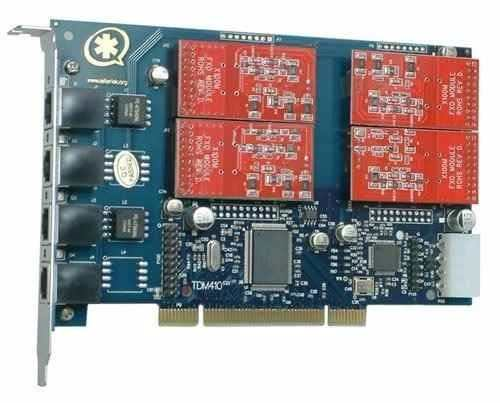
\includegraphics[width=8cm]{imagens/tdm410p.jpg}
	\caption{Placa TDM410P 4 portas.}
    \label{Figura16}
\end{figure}

\subsection{Rede de Computadores}
A LAN (\textit{Local Area Network}) ou rede de computadores local deve receber uma atenção especial desde o momento do projeto para a implementação de serviços com base VoIP, pois, a qualidade do áudio trafegado é afetado por fatores diretamente ligados à rede como o tamanho da banda, latência e jitter \cite{andersonramires2005}.

A rede de computadores do teleatendimento é composta por cabos de par trançado de categoria 5, e é interligada através de switch central com barramento 10/100 de 24 portas, e nas estações de trabalho (\textit{computadores}) o barramento das placas ethernet (\textit{placa de rede}) é de 10/100. A ilsutração do switch interligando as estações de trabalho pode ser vista através da figura \ref{Figura17}

\begin{figure}[h]
	\centering
	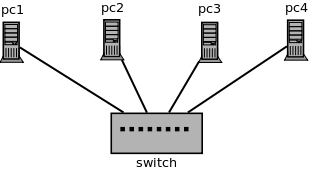
\includegraphics[width=8cm]{imagens/switch.png}
	\caption{Conexão entre o switch e as estações de trabalho.}
    \label{Figura17}
\end{figure}

\subsection{Hardware}
O teleatendimento não possui um computador exclusivo para a ferramenta Asterisk, então foi adquirido um computador com configurações razoáveis porém compatível com o cenário pretendido. O hardware foi escolhido acima do dimensionamento pretendido para o cenário, pois devido ao teleatendimento possuir somente quatro ramais analógicos, logo poderá ter somente quatro chamadas simultâneas. \citeonline{alexandrekeller2014} expõe que a quantidade de chamadas simultaneas e se ira gravar as chamadas e velocidade do disco são fatores para dimensionamento correto do hardware. 

\begin{figure}[h]
	\centering
	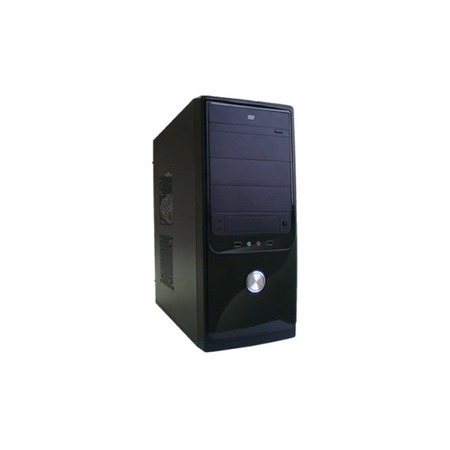
\includegraphics[width=6cm]{imagens/gabinete.jpg}
	\caption{Computador para o servidor PABX.}
    \label{Figura18}
\end{figure}

\subsection{Software}
O sistema operacional\footnote{Um sistema operacional é um conjunto de programas básicos e utilitários que fazem seu computador funcionar} escolhido para a instalação da ferramenta Asterisk foi a ultima versão estável do GNU/Linux Debian. O Debian é um sistema operacional de distribuição não comercial e livre que usa o kernel Linux. A versão oito do Debian com codinome Jessie é sua ultima versão estável, os desenvolvedores do Debian sempre homanegencia suas versões com nomes dos personagens do filme Toy Story\footnote{Toy Story é um filme estadunidense de aventura e comédia de 1995. É conhecido por ser o primeiro longa-metragem dos estúdios Pixar e também o primeiro da história totalmente feito por computação} \cite{valessiosoaresbrito2015}.

Além de ser um sistema operacional de distribuição livre, o Debian é uma distribuição de alta qualidade, estável e escalável, que podem ser facilmente configurado para servir em vários papéis, desde firewalls dedicadas a ambientes de estações de trabalho científico e até servidores de rede de elevada gama, e é especialmente popular entre utilizadores mais avançados devido à sua excelência técnica e ao seu profundo compromisso com as necessidades e expectativas da comunidade Linux \cite{valessiosoaresbrito2015}.



%%========================= CAPITULO 4 ==============================

\chapter{Aplicação} %\label{cap_exemplos}
%\thispagestyle{empty}
\section{Instalação do Asterisk}
A instalação do Asterisk requer e exige uma série de cuidados e detalhes,  para que se tenha um ambiente de telefonia estável e disponível o maior tempo possível. Logo, e necessário uma instalação onde busca-se a menor quantidade de problemas e com maior tempo operando, pois a compilação do Asterisk não é um processo trivial \cite{alexandrekeller2014}.

Apesar de haver duas formas de instalação, onde pode ser por SVN\footnote{Sistema de controle de versão} que mantêm um compartilhamento do desenvolvimento do sistemas com todas as novas funcionalidades, porém ainda nem sempre devidamente testadas, logo optou-se por baixar os pacotes compactados sendo eles:

\begin{itemize}
  \item dahdi-linux-current.tar.gz
  \item dahdi-tools-current.tar.gz
  \item libpri-1.4-current.tar.gz
  \item openr2-1.3.3.tar.gz
  \item libss7-1.0.2.tar.gz
  \item asterisk-13-current.tar.gz
\end{itemize}

E podem ser obtidos respectivamente nos seguintes endereços:

\begin{itemize}
  \item http://downloads.asterisk.org/pub/telephony/dahdi-linux/
  \item http://downloads.asterisk.org/pub/telephony/dahdi-tools/
  \item http://downloads.asterisk.org/pub/telephony/libpri/
  \item https://code.google.com/p/openr2/downloads/list
  \item http://downloads.asterisk.org/pub/telephony/libss7/
  \item http://downloads.asterisk.org/pub/telephony/asterisk/
\end{itemize}

Após o download dos mesmo foram descompactados e compilados na  mesma ordem em foram baixados, pois, os modulos são independentes, ou seja, a compilação de um módulo reflete diretamente na compilação do outro, a exemplo que caso seja compilado o módulo do Asterisk antes do módulo LIBPRI, a compilação do Asterisk não reconhecerá as funções habilitadas pelo pacote LIBPRI.

Após a instalação do Asterisk algumas pastas e arquivos são criados por ele para sua respectiva configuração e armazenamento das informações, pois o Asterisk é dividido em módulos, cada um representando uma funcionalidade como aplicação, função, canal de comunicação, protocolo e outros, e para correta configuração destas funcionalidades e necessário correta construção e configuração destes arquivos, e no decorrer do projeto, serão abordados os arquivos de configuração pertinentes para a correta construção do protótipo para ser testado no teleatendimento.

\subsection{Protótipo}
O protótipo consiste na construção de servidor PABX híbrido para o teleatendimento da Polícia Miltar de Dourados, onde será configurado as funcionalidades do Asterisk pertinentes a este teleatendimento, logo, será apresentado os arquivos com as configurações necessárias para esta finalidade.

\subsubsection{Plano de Discagem}
O plano de discagem define todo o funcionamento do servidor Asterisk, é onde define os grupos e regras de discagem, ou seja, como as chamadas de entradas e saída do servidor serão tratadas, e quais funcionalidades serão atividades e como funcionarão, o arquivo onde é programado o plano de discagem é o extensions.conf e fica localizado dentro da pasta /etc/asterisk/ \cite{alexandrekeller2014}.
Na figura 18 podemos observar como ficou sua configuração para o ambiente escolhido.

%%========================= CAPITULO 5 ==============================

\chapter{Conclusão e Trabalhos Futuros} %\label{cap_exemplos}
%\thispagestyle{empty}
Através deste projeto foi possível, a partir dos estudos teóricos e práticos sobre a telefonia convencional, VoIP, e a ferramenta Asterisk, elaborar, configurar e testar através de um protótipo, ou seja, demonstrar que é possível aplicar inteligencia computacional neste teleatendimento e ainda proporcionar segurança e confiança aos atendentes e cidadãos douradenses com relação ao teleatendimento da Polícia Militar.

O trabalho desempenhado ainda demonstrou, além de um estudo teórico para levantamento bibliográfico, o desenvolvimento prático de uma servidor PABX, é capaz de prover comunicação em um ambiente misto de telefonia, onde o usuário, localizado em algum ponto da telefonia pública (PSTN), se comunica com a rede de dados com ramais VoIP. A partir do efetivo funcionamento deste servidor foi possível, de maneira prática, agregar valor ao sistema de telefonia do teleatendimento.

Este trabalho conseguiu-se contribuir no sentido de enriquecer e agregar conhecimento a este tema, até então, pouco explorado pela comunidade científica. Demonstrou-se também inovador, pois foi elaborado um protótipo de servidor com funcionalidades pertinentes a um setor de teleatendimento emergencial de um órgão de segurança publica.

A implementação do protótipo no teleatendimento foi autorizado pelo diretor técnico do CIOPS, o qual acompanhou alguns testes realizados com o protótipo. E após esta etapa, o cenário apresentado foi aprovado pelo mesmo e os integrantes do teleatendimento que puderam acompanhar os testes realizados.

Como trabalhos futuros, sugere-se que sejam realizados testes no ambiente, fazendo uso de hardware específico para a comunicação do ambiente baseado em VoIP com a telefonia convencional, afim de verificar a sua estabilidade e eficiência. Também como trabalhos futuros, visa-se ampliar o número de informações monitoradas nos servidores e também aumentar o número de servidores monitorados, a fim de calcular a demanda de fluxo gerado por estes na
rede de dados.

Como trabalhos futuros, sugere-se que sejam realizados testes de integração com o servidor VoIP e as viaturas que possuírem algum dispositivo móvel conectado a internet, para verificar a possibilidade de teleconferência entre os atendentes e as viaturas bem como o cidadão a qual originou a chamada ao teleatendimento.

Com o ambiente de telefonia em pleno funcionamento, sugere-se também o desenvolvimento de um número maior de aplicações, como a personalização da bilhetagem, mas informações podem ser guardadas. E a possibilidade da criação ou mesmo reaproveitação de softphone com código fonte aberto, para personalização para teleatendimento, a exemplo onde após um atendimento o atendente possa colocar a chamada como sendo realmente um atendimento, trote ou pedido de informação.


% ----------------------------------------------------------
% Finaliza a parte no bookmark do PDF
% para que se inicie o bookmark na raiz
% e adiciona espaço de parte no Sumário
% ----------------------------------------------------------
\phantompart

% ----------------------------------------------------------
% ELEMENTOS PÓS-TEXTUAIS
% ----------------------------------------------------------
\postextual
% ----------------------------------------------------------

% ----------------------------------------------------------
% Referências bibliográficas


%==================== REFERENCIAS BIBLIOGRAFICAS =====================
\renewcommand{\refname}{Referências Bibliográfica}
\bibliography{refbib}   % Bibliografia
%\thispagestyle{empty}

%============================== ANEXOS ===============================
%\anexo
%\chapter{Título do anexo}


%---------------------------------------------------------------------
% INDICE REMISSIVO
%---------------------------------------------------------------------
\phantompart
\printindex
%---------------------------------------------------------------------


\end{document}

% ------- Fim do Pre\^{a}mbulo - Inicio do Documento --------